\chapter{Results} % Main appendix title

This appendix contains notes related to obtaining results that were and were not used in the final dissertation. Results that were not used are left for completeness, as they may be used for future work.

\label{AppendixD} % For referencing this appendix elsewhere, use \ref{AppendixX}

\section{Ford AV Dataset steering angles}

\subsection{Ford AV Dataset}

The steering angles can be extracted from .bag files using ROS commands:
\begin{verbatim}
    # In one terminal, start ros engine
    $ roscore
    # In another terminal, inspect content of bag file
    $ time rosbag info Sample-Data.bag
    (...)
             /imu                 146939 msgs    : sensor_msgs/Imu             
    (...)
             /pose_ground_truth   146136 msgs    : geometry_msgs/PoseStamped   
             /pose_localized       16100 msgs    : geometry_msgs/PoseStamped   
             /pose_raw            146190 msgs    : geometry_msgs/PoseStamped   
(...)
    # And subscribe to topic of interest 
    $ rostopic echo /imu | tee sample_imu.yaml
    # In another terminal, playback bag file
    $ time rosbag play --immediate Sample-Data.bag --topics /imu
    # Sanity check, count number of acquisitions
    $ cat sample_imu.yaml | grep "orientation:" | wc -l
\end{verbatim}
The snippet above generates file imu.yaml, with all pose data generated by imu device. From this file we extract the steering angle, which is the z axis (yaw) of the orientation field (TODO check .yaml dialect). 
Images can be extracted from the same bag file with the Python 2.7 bag\_to\_images.py script:
\begin{verbatim}
    $ python2 bag_to_images.py Sample-Data.bag ~/git/msc-data/ford/sample/ros/ \
        /image_front_left
\end{verbatim}
Each image is an attribute in a dictionary, which also contains seconds (secs) and nano seconds (nsecs) attributes within the header attribute:
\begin{verbatim}
header: 
  seq: 213414
  stamp: 
    secs: 1501822147
    nsecs: 684951066
  frame_id: "camera_front_left"
height: 215
width: 414
encoding: "8UC3"
is_bigendian: 0
(...)
\end{verbatim}
Thus a timestamp can be obtained for each image extracted. This is done with script  
  
parse\_yaml\_time.py:
\begin{verbatim}
$ python ./ford/sample/parse_ford_yaml_time.py
header -> {'seq': 213414, 'stamp': {'secs': 1501822147, 'nsecs': 684951066}, 'frame_id':
'camera_front_left'}
1501822147,684951066
header -> {'seq': 213415, 'stamp': {'secs': 1501822147, 'nsecs': 820741891}, 'frame_id':
'camera_front_left'}
1501822147,820741891
(...)
\end{verbatim}
While the steering angles are extracted (TODO ADD QUATERNION CORRESPONDENCE)
The image can be matched with a steering angle by obtaining the timestamp of image, the full secs 

\section{Audi}

The  Audi Autonomous Driving Dataset (A2D2)
authors (\cite{geyer2020a2d2}) are motivated by the fact that research in machine learning, mobile robotics and autonomous driving is accelerated by the availability of high quality annotated data. This statement can be verified by the advances in image classification with deep neural networks since \cite{IMAGENET} became available.  
The A2D2 data was acquired with a human-driven Audi Q7 e-tron equipped with six cameras (front left, front center, front right, back left, back center, back right) and five LiDAR sensors. The authors claim this resulted in  360$^{\circ}$ camera and LiDAR coverage. Additionally, several bus data signals from the vehicle were recorded such as velocity, acceleration and steering wheel angle. 
The total size is 2.3TB. Our datasets of interest are the  Though, since we are interested in image and steering angle only, our data can be narrowed to 
\begin{verbatim}
https://aev-autonomous-driving-dataset.s3.eu-central-1.amazonaws.com/
README-SensorFusion.txt
    
- steering_angle_calculated
- steering_angle_calculated_sign

- 'cam_front_center'
\end{verbatim}

The dataset total size is approximately 2.3TB, although the majority is sensor fusion data note used in this study. The data can be dwonloaded from   
  
\url{https://www.a2d2.audi/a2d2/en/download.html}

This was supplied for three cities: Gaimersheim, Ingolstadt and Munich. To perform initial investigations we chose data from Munich and downloaded the "Camera - Front Center" images, constituting 27451 images 3.2MB in size each and dimension 1920x1208 pixels, total size on disk is about 92GB. We also downloaded the 176MB "Bus Signals" file. The image naming convention uses a timestamp in the format:
\begin{verbatim}
20190401145936_camera_frontcenter_000017970.png
\end{verbatim}
The "Bus Signals" file is JSON encoded and provides several signals such as acceleration, angular velocity and vehicle speed. Our signals of interest are the steering angle calculated and steering angle sign. In the bus signals file (20190401121727\_bus\_signals.json) we parsed our values of interest e.g.
\begin{verbatim}
(...)
    "steering_angle_calculated": {
        "unit": "Unit_DegreOfArc",
        "values": [
            [
                1554115464698116,
                2.4
            ],
(...)
\end{verbatim}
where the unit is degree of arc and the values are inferred to be a timestamp when the measurement was acquired and the angle (1554115464698116 and 2.4 respectively, in the example shown).
and found 91968 entries for each of the steering angle and sign. This is over 3 times the amount of corresponding images. Since there was no obvious key to match the steering angle and sign with a corresponding image, we wrote to the supplied enquiry email address aevdrivingdataset@audi.de with regard to this problem and receiving no reply, abandoned the dataset deeming it unusable for our purposes.  
Note: we did try converting the integer into a date using python, which resulted in an error:
\begin{verbatim}
import datetime
audi_timestamp = 1554115464698116
date = datetime.datetime.fromtimestamp(audi_timestamp / 1e3)
print(date)
# ValueError: year 51217 is out of range    
\end{verbatim}
(TODO ADD CORRESPONDENCE WITH AUTHOR)

%% TODO add correspondence with Mentar

\section{Unity3D changing sky hue}
The simulator is started by running:
\begin{verbatim}
$ sudo ~/.Unity.AppImage --no-sandbag   
\end{verbatim}
This will load the Unity Hub application. A project can be added, which will be repository cloned from \cite{SDSandboxSim}. Once loaded, the menu scene is selected and the project is run. Once running, an output directory must be chosen. A track is then selected (TODO track list), then the option "Auto with REC TODO double check".  
TODO ADD IMAGE SEQUENCE  
Once a number of laps have been completed, the images can be moved to a labelled folder using prepare\_data.py script. This will move images to a user defined directory, create a sub-directory named with a date and timestamp

The sky colour can be changed via Window > Renderering > Lighting settings, then under Environment changing "Skybox Material". Default Skybox Material is "Default-Skybox". Suggested for darker background is "Usa\_Number\_M" - blue.

Changing camera sensor image output size

There are two ways to change the size of images output by simulator camera sensor, one is by editing Donkey.Prefab file and changing lines 3415 and 3416:
\begin{verbatim}
  width: 160
  height: 120
\end{verbatim}
The other was is through Unity
Changing sky colour
The sky colour can be changed via Windows > Renderer > Lighting Settings menu, then under Environment changing "Skybox Material" chossing a different material.  Suggested for darker background is "Usa\_Number\_M".
The simulator lighting can be made darker, in the same menu, under Environment Lighting > Intensity MUltiplier. A value of 1 is chosen to generate training datasets, and a value of 0.26 when running the simulator in NN Control over Network mode, that is using the prediction engine to predict steering angles.
\section{Udacity}

1. Link trail - medium (Indian guy) -> medium (Chinese guy)-> github (Japanese guy)  
  
2. Udacity data  
Data is available for download in torrent file format (\cite{torrentCite}) and consist of Robot Operating System (ROS) rosbag compressed files.

\begin{verbatim}
https://github.com/udacity/self-driving-car/tree/master/datasets
\end{verbatim}
3. Rosbag

\section{utbm}
More stuff from german uni? TODO ADD AND COMPLETE OR REMOVE
\begin{verbatim}
https://epan-utbm.github.io/utbm_robocar_dataset/
\end{verbatim}

\section{Training and Testing Log}

The first two entries are incomplete, have been commented out and can be seen in the latex AppendixD-results.tex file.
%\begin{verbatim}
%Run ID  Data       Network Acc. Error Saved Best Model 
%3       log_sample NVIDIA1
%\end{verbatim}

%Run ID  Data    Network Training    Acc Error   Saved Best Model    Saved History
%1       Udacity 1       SGD Adam    .95 .06     model_01            history_01

\subsection{Run 3}

This model has a single output, steering angle, and produced very low accuracy.
Notes:
\begin{verbatim}
commit 423b5b783565b60e72f970485d9b3aa9887f5453
training time
dataset: sample_data
\end{verbatim}

\subsection{Run 4 - }

% Naoki's model not doing well, sanity check with one output
Also not doing well
Next run, 2 outputs (steering and throttle)

\subsection{Run 5 - 20201102081239} 

\begin{verbatim}
commit 076e8b32664738df6af9e14d75355504eb2a94b4
Much better results with two outputs. 
cat ../dataset/unity/log_sample/logs_Mon_Jul_13_08_29_01_2020/record_11659.json
Both are floats - steering angle and throttle
loss: 0.0105 - acc: 0.8502 - val_loss: 0.0111 - val_acc: 0.8617

dataset: sample_data
model: nvidia1
outputs: 2

Comment: Network trained with no augmentation of cropping.

\end{verbatim}

From this point onwards, a model name, if generated, is given with every run.

\subsection{Run 5 - 20201102090041\_nvidia2}
\begin{verbatim}
commit 42dabb6321ad25f667c8663b63412c88c96b3b38
model: nvidia2
outputs: 2
dataset: log_sample (size: 12k)
$ python train.py --model=nvidia2 --outdir=../trained_models
loss: 0.0108 - acc: 0.8483 - val_loss: 0.0117 - val_acc: 0.8495
\end{verbatim}

\subsection{Run 6 - 20201102094552\_nvidia1}
\begin{verbatim}
commit ec9d081b85f7386365428a73896b1d09be7ba917
model: nvidia1
outputs: 2
dataset: genRoad (280727)
command
$ train.py --model=nvidia1 --outdir=../trained_models
loss: 0.0077 - acc: 0.8726 - val_loss: 0.0077 - val_acc: 0.8732

Comment: Network trained with no augmentation of cropping.

video upload: https://youtu.be/ZLhrcyuONj0
\end{verbatim}

\subsection{Run 7 - 20201102090041\_nvidia2.h5}
\begin{verbatim}
commit 1da10b6745f583e180d5b9c5ba4874847ba8610c
model: nvidia2
outputs: 2
Dataset: genRoad
command
$ train.py --model=nvidia2 --outdir=../trained_models
\end{verbatim}

\subsection{Run 8 - 20201102134802\_nvidia2.h5}
\begin{verbatim}
commit 6960f2f5fb50b565c0dfd6c8fe3ac1d283192e69
model nvidia2
outputs 2
dataset log2
command:
train.py --model=nvidia2 --outdir=../trained_models
\end{verbatim}


\subsection{Run 9 - 20201102210514\_nvidia2.h5}
\begin{verbatim}
Running nvidia2 with augmentation
commit 6960f2f5fb50b565c0dfd6c8fe3ac1d283192e69
model nvidia2
outputs 2
dataset log2
command:
train.py --model=nvidia2 --outdir=../trained_models
loss: 0.0345 - acc: 0.7906 - val_loss: 0.0236 - val_acc: 0.8084
Stop! Still running!!! Epoch 60 and still improving. ...
% loss: 0.0193 - acc: 0.8250 - val_loss: 0.0116 - val_acc: 0.8503
% 0.0123 - acc: 0.8501 - val_loss: 0.0091 - val_acc: 0.8594
Ran 78 epochs and may have thrown error:
problems with loss graph
Note biggest increase in accuracy during training
\end{verbatim}

\subsection{Run 10 - 20201103211330\_nvidia2.h5}
\begin{verbatim}
Run nvidia2 WITHOUT augmentation, just preprocessing
commit 2add77bb60505fe25075f9da55f6465e65cd3825
model nvidia 2
outputs 2
dataset log2
command:
train.py --model=nvidia2 --outdir=../trained_models
loss: 0.0233 - acc: 0.8179 - val_loss: 0.0170 - val_acc: 0.8304
loss: 0.0084 - acc: 0.8656 - val_loss: 0.0086 - val_acc: 0.8655
Epoch 45/100
loss: 0.0083 - acc: 0.8662 - val_loss: 0.0086 - val_acc: 0.8638
problems with loss graph

No loss graph, again, no augmentation trained quicker that previous

\end{verbatim}

\subsection{Run 11}
\begin{verbatim}
commit 6439a8758d8b46a1cbc3bcefc9db4c15f70820df
model nvidia1
outputs 2
dataset log2
command:
train.py --model=nvidia1 --outdir=../trained_models
Epoch 1/100
1755/1755 [==============================] - 682s 389ms/step - loss: 0.0271
- acc: 0.8049 - val_loss: 0.0172 - val_acc: 0.8351
Epoch 84/100
1755/1755 [==============================] - 559s 318ms/step - loss: 0.0099 
- acc: 0.8581 - val_loss: 0.0083 - val_acc: 0.8662
problems with loss graph (probably a bug introduced in adding info to graph?)

\end{verbatim}

\subsection{Run 12}
\begin{verbatim}
commit augment.ipynb
model nvidia_baseline
outputs 1
dataset log2 (280746)
command:
train.py --model=nvidia_baseline --outdir=../trained_models

There is an issue with the aspect ratio and cropping, need to investigate with
augment.ipynb

Note unity dataset log2 was renamed genRoad as it is obtained from a number of
randomly generated Generated Road circuits.

\end{verbatim}

\subsection{Run 13}
\begin{verbatim}
commit e14e4bb9bdd0d322867c6cdba706478f662e71f6
model nvidia_baseline
outputs 1
dataset log (45421)cd 
command:
train.py --model=nvidia_baseline
--outdir=../trained_models
--epochs=1
--inputs=../dataset/unity/log/*.jpg
--aug=True
--preproc=True

Comment: ran ok for one epoch, images sized correctly.
Adding more epochs
\end{verbatim}

\subsection{Run 14}
\begin{verbatim}
commit e14e4bb9bdd0d322867c6cdba706478f662e71f6
model nvidia_baseline
outputs 1
dataset log
command:
train.py --model=nvidia_baseline
--outdir=../trained_models
--epochs=100
--inputs=../dataset/unity/log/*.jpg
--aug=True
--preproc=True

Comment: Started with very low accuracy.
Stopped process as error seems to have gone out of range
Epoch 5/100
283/283 [==============================] 
- 107s 377ms/step - loss: nan - acc: 5.5259e-05 
- val_loss: nan - val_acc: 1.1004e-04
\end{verbatim}

\subsection{Run 15}
\begin{verbatim}
commit aec3290fdbc83e71e450deef650aa2d51873b886
model nvidia_baseline
outputs 2
dataset log
command:
train.py --model=nvidia_baseline
--outdir=../trained_models
--epochs=100
--inputs=../dataset/unity/log/*.jpg
--aug=True
--preproc=True
Comment: Started at loss: nan - acc: 0.4305. Two outputs definitely help. Why?
Perhaps because model is not going around track at constant speed?

\end{verbatim}

\subsection{Run 16}

\begin{verbatim}
commit 10a3fc2f6d23e04f604914c1f8420e574a8ce808
model nvidia_baseline
outputs 2
dataset log
command:
train.py --model=nvidia_baseline
--outdir=../trained_models
--epochs=100
--inputs=../dataset/unity/log/*.jpg
--aug=True
--preproc=True
Comment: Added linear activation in final layer, loss returning a reasonable value:
loss: 1.2035 - acc: 0.5404
Turned into nan on 3rd epoch. Accuracy going down, stopping process
\end{verbatim}

\subsection{Run 17}

\begin{verbatim}
Commit: a76169106a9087f5cc7e851fe09294699bb6240c 
Model: nvidia_baseline
Outputs: 2
Dataset: genRoad
Command: 
train.py --model=nvidia_baseline
--outdir=../trained_models
--epochs=100
--inputs=../dataset/unity/log/*.jpg
--aug=True
--preproc=True

Comment: Removed weight decay
Still loss taking NaN values
Epoch 13/100
281/281 (...) val_loss: nan - val_acc: 0.4939

\end{verbatim}

\subsection{Run 18 }

\begin{verbatim}
Commit: baa8f3d066dc37d3c2bb7792fa9db4801824d1bb 
Model: nvidia_baseline
Outputs: 2
Dataset: genRoad
Command: 
train.py --model=nvidia_baseline
--outdir=../trained_models
--epochs=100
--inputs=../dataset/unity/log/*.jpg
--aug=True
--preproc=True
Comment: Removed dropout from last dense layer. Training loss NaN on first epoch.
Dropout added again, loss back to under 1. Seems to have an influence, trying
multiple dropout removals next.

\end{verbatim}



\subsection{Run 19}
\begin{verbatim}
Commit: 16a6f8ffc6399143e7ad5a6885ee9b44b3ca1dda
Model: nvidia_baseline
Outputs: 2
Dataset: genRoad
Command: 
train.py --model=nvidia_baseline
--outdir=../trained_models
--epochs=100
--inputs=../dataset/unity/log/*.jpg
--aug=True
--preproc=True
Comment: Left one dropout (.25) layer, loss still NaN.
\end{verbatim}

\subsection{Run 20}

\begin{verbatim}
Commit: d7e05ad1cdf0fab3a83975be259feb16830b5a38
Rest same as 19
Comment: Removed Dense(1164) layer. Loss is Nan on first epoch.
Stopping run

\end{verbatim}

\subsection{Run 21}
\begin{verbatim}
Commit: d8fb9705dd676554dcf84a213b3c27d0e1f9d0c4 
Rest same as 19
Comment: Loss is Nan on first epoch
Epoch 1/100
(...)loss: nan - acc: 0.5017
\end{verbatim}

\subsection{Run 22}
\begin{verbatim}
Commit: ba4432568a589eac5a7d7c4927fa96e2f9e11bd1
Model, Outputs, Dataset and Command: Same as 19
Comment: Using Glorot Uniform (Xavier) kernel initializer.
Loss in Nan on first epoch. Training stopped.
Epoch 1/100
284/284 [==============================] - 101s 357ms/step - loss: nan 
- acc: 0.4609
\end{verbatim}

\subsection{Run 23}
\begin{verbatim}
Commit: 5cba2c7b01a160e7053e09220e63b1c575cf51e8  
Model, Outputs, Dataset and Command: Same as 19
Comment: All biases initialized to 0.
Loss in Nan on first epoch. Training stopped.
Epoch 1/100
283/283 (...) loss: nan 
\end{verbatim}

\subsection{Run 24}
\begin{verbatim}
Commit: 56aea3e16bb0f9db5735dfa536809389f35b12da  
Model, Outputs, Dataset and Command: Same as 19
Comment: Removed Dense(10) layer
Loss in Nan on first epoch. Training stopped.
\end{verbatim}

\subsection{Run 25}
\begin{verbatim}
Commit: 6a8ee72727db2508d2ff1ae35d068837a5b524ab  
Model, Outputs, Dataset and Command: Same as 19
Comment: Increased dropout to 0.5.
Loss in Nan on second epoch. Training stopped.
Epoch 1/100
285/285 [==============================] - 100s 352ms/step 
- loss: 0.0660 - acc: 0.6910 - val_loss: 0.0299 - val_acc: 0.7809
Epoch 2/100
285/285 [==============================] - 100s 350ms/step - loss: nan 
- acc: 0.5000
\end{verbatim}

\subsection{Run 26}
\begin{verbatim}
Commit: e4a287dc816a2a4d2c47893b131c710b2ecb8594  
Model, Outputs, Dataset and Command: Same as 19
Comment: Spreading 0.5 dropout between layers (0.1 each).
Loss in Nan on third epoch. Training stopped.
Epoch 3/100
284/284 (...) loss: nan
\end{verbatim}

\subsection{Run 26}
\begin{verbatim}
Commit: 2e5bf1b7002a2ddbbe2fea003fce010627d723e2  
Model, Outputs, Dataset and Command: Same as 19
Comment: Changed layer dropout to 0.15.
Loss in Nan on first epoch. Training stopped.
\end{verbatim}

\subsection{Run 27}
\begin{verbatim}
Commit:   
Model, Outputs, Dataset and Command: Same as 19
Comment: Changed layer dropout to 0.05.
Loss in Nan on first epoch. Training stopped.
\end{verbatim}

\subsection{Run 28}
\begin{verbatim}
Commit: 9a70ff7e194736a475bdce0b6eddc65aad6ea8c0  
Model, Outputs, Dataset and Command: Same as 19
Comment: Changed number of kernels on 2nd Conv layer to 32.
Loss in Nan on first epoch. Training stopped.
\end{verbatim}

\subsection{Run 29}
\begin{verbatim}
Commit:   
Model, Outputs, Dataset and Command: Same as 19
Comment: Changed number of kernels on 3nd Conv layer to 64.
Loss in Nan on first epoch. Training stopped.
\end{verbatim}

\subsection{Run 30}
\begin{verbatim}
Commit: 1997b914e829466659a27bfe1b31a6a6374afd36  
Model, Outputs, Dataset and Command: Same as 19
Comment: Changed aspect ratio to 160x120
Loss in Nan on 2nd epoch. Training stopped.
Epoch 2/100
283/283 (...) loss: nan - acc: 0.5982
\end{verbatim}

\subsection{Run 31}
\begin{verbatim}
Commit: 1997b914e829466659a27bfe1b31a6a6374afd36  
Model, Outputs, Dataset and Command: Same as 19
Comment: Changed aspect ratio to 160x120
Loss in Nan on 2nd epoch. Training stopped.
Epoch 2/100
283/283 (...) loss: nan - acc: 0.5982
\end{verbatim}

\subsection{Run 32 - 20201117154210\_nvidia\_baseline.h5}
\begin{verbatim}
Commit: 1997b914e829466659a27bfe1b31a6a6374afd36  
Model: nvidia_baseline
Outputs: 2
Dataset: smallLoopingCourse (jungle1 renamed) (34443)
Command: 
train.py --model=nvidia_baseline
--outdir=../trained_models
--epochs=100
--inputs=../dataset/unity/genTrack/log/*.jpg
--aug=True
--preproc=True
Comment: Loss in Nan on 1st epoch. Training stopped.
This run also produced a usable model.
\end{verbatim}

\subsection{Run 33}
\begin{verbatim}
Commit: 861095ac1a997e0f460aca6ceda93df98b7d0a48  
Model, Outputs, Dataset and Command: Same as 19
Comment: Explicitly setting strides=(1,1) is conv layers 4 and 5.
Loss in Nan on 1st epoch. Training stopped.
\end{verbatim}

\subsection{Run 34 - 20201117162326\_nvidia\_baseline.h5}
\begin{verbatim}
Commit: d0b7160793ee433ed25724d966a7d3bd85ae8ffa  
Model, Outputs, Dataset and Command: Same as 19
Comment: Changed batch size to 64
Loss is NaN on 7th epoch
Epoch 7/100
567/567 (...) loss: nan

This run produced a usable model.
\end{verbatim}

This run consisted of a sanity check to determine if training would generate a loss value different from NaN (not a number). This was not the case as per results in comments.

\subsection{Run 35 - 20201120124421\_nvidia\_baseline.h5}
\begin{verbatim}
Commit: 1f5c64bc219b31cf8654d2cceec910f0dea5ecbf
Model: nvidia_baseline
Outputs: 2
Dataset: log_sample (12894 - small looping track)
Environment: simbox (local)
Command: 
--model=nvidia_baseline --outdir=../trained_models --epochs=100
--inputs=../dataset/unity/log_sample/*.jpg --aug=True --preproc=True

Comment: Sanity check run, with the aim of
establishing a repeatable training session, aiming
at debbugging Keras when the need arises, that is
when Keras is suspected of somehow having become 
corrupted. 

Note before running, all .jpg images were found to have corresponding 
steering angles:

$ python ~/git/sdsandbox/src/utils/jsonclean.py \
--inputs=/home/simbox/git/sdsandbox/dataset/unity/log_sample/*.jpg
Files deleted: 0

From the log file 20201120124421\_nvidia\_baseline.log:

Total training time: 0:03:09
Training loss: nan
Validation loss: nan
Training accuracy: 0.418
Validation accuracy: 0.480

Loss was NaN from 2nd training epoch:
Epoch 2/100
160/160 (...)- loss: nan

When running the model:

sudo ./Unity.AppImage --no-sandbox
And logging the session:
sudo tcpflow -i lo -c port 9091 > /tmp/tcpflow.log
and running predictions
python predict_client.py
--model=../trained_models/nvidia_baseline/20201120124421\_nvidia\_baseline.h5

The model was found to crash into a bollard. A video was generated using 
src/utils.MakeVideo.py

https://youtu.be/ZwP53IhBO20

\end{verbatim}

Given previous results, this run reverts code to commit 436f635f

%%%%%%%%%%%%%%%%%%%%%%%%%%%%%%%%%%%%%%%%%%%%%%%%%%%%%%%%%%%%%%%%%%%%%%%%%%%%%
% RUN 36
%%%%%%%%%%%%%%%%%%%%%%%%%%%%%%%%%%%%%%%%%%%%%%%%%%%%%%%%%%%%%%%%%%%%%%%%%%%%%
\subsection{Run 36 - 20201120171015\_sanity.h5}
(Referenced from \ref{results:net-training})
Long story short: Forensics are conducted in this run to find out what code generated model 
20201107210627\_nvidia1.h5, determining that outliers present in genRoad create problems. The outliers have since been quarantined.

\label{app_res:36}

\begin{verbatim}
Commit: 436f635fa183740832270ea7db6869918a786d55
Model: nvidia1
Outputs: 2
Dataset: log_sample (12894) 
Command: python train.py --model=sanity --outdir=../trained\_models
Environment: simbox
Comment: This model was trained with the committed code from November 7th, which
produced the first success lap drive with not crashes or steering off the track.
There is no record of what commit generated the model, though on video:
https://youtu.be/9z0mMtOnUUc
One section in the video shows:
python predict_client.py \
--model=../trained_models/nvidia1/20201107210627\_nvidia1.h5
The model name contains date and time created.

The sanity check model trained in under five minutes, and the best model saved 
was most likely (subject to double checking Keras source code) generated on the
third epoch.

cat 20201120171015_sanity.log
Model name: ../trained_models/sanity/20201120171015_sanity.h5
Total training time: 0:04:38 (...)

A record of the training output is displayed below:

Epoch 1/100
80/80 [==============================] - 35s 432ms/step - loss: 0.0822 
- acc: 0.6293 - val_loss: 0.0300 - val_acc: 0.8109
Epoch 2/100
80/80 [==============================] - 34s 425ms/step - loss: 0.0650 
- acc: 0.7127 - val_loss: 0.0264 - val_acc: 0.8129
Epoch 3/100
80/80 [==============================] - 34s 423ms/step - loss: 0.0539 
- acc: 0.7429 - val_loss: 0.0276 - val_acc: 0.8133
Epoch 4/100
80/80 [==============================] - 34s 424ms/step - loss: nan 
- acc: 0.5398 - val_loss: nan - val_acc: 0.4930
Epoch 5/100
80/80 [==============================] - 34s 427ms/step - loss: nan 
- acc: 0.4228 - val_loss: nan - val_acc: 0.4910
Epoch 6/100
80/80 [==============================] - 34s 428ms/step - loss: nan 
- acc: 0.4245 - val_loss: nan - val_acc: 0.4963
Epoch 7/100
80/80 [==============================] - 34s 431ms/step - loss: nan 
- acc: 0.4216 - val_loss: nan - val_acc: 0.4934
Epoch 8/100
80/80 [==============================] - 34s 428ms/step - loss: nan 
- acc: 0.4285 - val_loss: nan - val_acc: 0.4922

Further forensic examination of commits:

Trying to find what data and code generated model 20201107210627_nvidia1.h5
This was generated on November 7th. There are 4 commits for that day:

src(master)$ git log > gitlog.txt
src(master)$ vim gitlog.txt 
/Nov 7
ESC
:q

commit 436f635fa183740832270ea7db6869918a786d55 * commit used for this run
commit 9908eb32975fe33075fefad73f411896456b4a84 
commit 1ad187d4bff5b6936c065a1aaa15a654ef4d368c
commit 8ebd02ab9556a0c2869e9b551417a6e28d5f86cf

$ git diff master..436f635 train.py | grep "\-\-inputs"
-    parser.add_argument('--inputs', default='../dataset/unity/genRoad/log/*.jpg',
+    parser.add_argument('--inputs', default='../dataset/unity/log_sample/*.jpg', 

$ git diff master..9908eb3297 train.py | grep "\-\-inputs"
-    parser.add_argument('--inputs', default='../dataset/unity/genRoad/log/*.jpg' (...)
+    parser.add_argument('--inputs', default='../dataset/unity/log_sample/*.jpg' (...)

$ git diff master..1ad187d4b train.py | grep "\-\-inputs"
-    parser.add_argument('--inputs', default='../dataset/unity/genRoad/log/*.jpg'
+    parser.add_argument('--inputs', default='../dataset/unity/log2/*.jpg', 

$ git diff master..8ebd02ab train.py | grep "\-\-inputs"
-    parser.add_argument('--inputs', default='../dataset/unity/genRoad/log/*.jpg'
+    parser.add_argument('--inputs', default='../dataset/unity/log2/*.jpg',

The plus signal indicates lines added in the commit to the right, minus indicates
what does not exist in the commit to the right (9908eb3297) , where master is 
commit 436f635fa (current commit at time or forensic code analysis).

First two commits indicate log_sample dataset was used containing 38684 images 
files of
"small looping course" course
/log_sample(master)$ grep -nr jpg . | wc -l
38684
was used, 
second two commits indicate log2 dataset (renamed genRoad) containing 280747 
image files on the "Generated Road" course.
/genRoad(master)$ grep -nr jpg . | wc -l
280747 (files)

The commits are listed in descending  chronological order, that is the first 
two datasets used to train on that day were log2 (later renamed genRoad), the
following two datasets used were log_sample. The commit history suggests one
of the two were used to generate the Nov 7 successful model. Since the test 
was run on "Generated Track" course, and genRoad contains images for "Generated
Road" course, the assumption is sample_log dataset was used.

The sanity check model was then used to run predictions:
python predict_client.py 
--model=../trained_models/sanity/20201120171015_sanity.h5
(...)
connecting to 127.0.0.1 9091
fps 10.416671685462958
fps 10.405931675595545
fps 11.030877564739708
fps 11.092089084017463
fps 11.466601323987536
fps 11.362325028068517
fps 11.359920970581536
fps 10.861855550070638
fps 10.50113576298416
(...)

The tcpflow log was saved to:

tcpflow(master)$ ls
20201107210627_sanity_tcpflow.log

And a video generated (from /tmp copy) with script src/MakeVideo.py
$ python MakeVideo.py --filename=/tmp/tcpflow.log \ 
--model=20201120171015_sanity.h5 
and the video.avi output uploaded to https://youtu.be/JaSkkh-2xtI

Qualitatively (by observation) had a better lap than 20201107210627_nvidia1.h5 
(https://youtu.be/9z0mMtOnUUc) as it keeps to a single lane and the vehicle wheels
never touch the road markings

Noting that the prior predict_client.py fps logs indicate that frames-per-second 
at varying ratios (e.g. fps 10.50113576298416), while MakeVideo.py records at 11
frames per second.
The video generated by MakeVideo.py is going around the track slightly faster
than the SDSandbox simulator steering with 20201120171015_sanity.h5 predictions.
between logged frames (tcpflow) and rendered frames (MakeVideo.py).
The frame rate logged with tcpflow is the frame rate SDSandbox is sending frames over 
the TCP network.

\end{verbatim}

%%%%%%%%%%%%%%%%%%%%%%%%%%%%%%%%%%%%%%%%%%%%%%%%%%%%%%%%%%%%%%%%%%%%%%%%%%%%%
% RUN 37
%%%%%%%%%%%%%%%%%%%%%%%%%%%%%%%%%%%%%%%%%%%%%%%%%%%%%%%%%%%%%%%%%%%%%%%%%%%%%
\subsection{Run 37 - 20201120184912\_sanity.h5}
Referenced from \ref{results:net-training} 
\label{app_res:37}
\begin{verbatim}
Commit: 1ad187d4bff5b6936c065a1aaa15a654ef4d368c
Model: nvidia1
Outputs: 2
Dataset: log2 (genRoad)
Command: python train.py --model=sanity --outdir=../trained\_models
Environment: simbox
Comment: This was the 3rd commit of the day
It seems that this has something to do with the dataset that was
being used. To be confirmed. Now running nvidia1 on genRoad
both on simbox and camber, loss still converging to 0
and not in NAN range. 

Training log:  ../trained_models/sanity/20201120184912\_sanity.log
Total training time: 16:08:01
Training loss: 0.010
Validation loss: 0.008
Training accuracy: 0.858
Validation accuracy: 0.858

This model took over 16 hours to train on 280727 images. It did not perform well.
Could it be due to the outliers?

$ sudo tcpflow -i lo -c port 9091 > /tmp/tcpflow.log
$ python predict_client.py --model=../trained_models/sanity/20201120184912_sanity.h5
$ python MakeVideo.py --filename=/tmp/tcpflow.log --model=20201120184912_sanity.h5

The angles were plotted using notebook GetSteeringAnglesFromtcpflow.ipynb
sa = GetSteeringFromtcpflow('../dataset/unity/genRoad/tcpflow/20201120184912_sanity.log')
sarr = np.asarray(sa)
p = sarr[:,0]
g = sarr[:,1]
plotSteeringAngles(p, g, 25, False, "Generated Road", "20201120184912_sanity.h5")

\end{verbatim}
%PAUSE HERE - WRITING FUNCTION TO PLOT STEERING ANGLES AND BINS FROM LOGS
Below are the normalized histogram and bins recovered from tcplow logs for model  
  
20201120184912\_sanity.h5 referenced in \ref{results:net-training}. The video generated from tcpflow log was uploaded to \href{https://youtu.be/xGDN8qOnv9M}{https://youtu.be/xGDN8qOnv9M}.

\begin{figure}[ht]
 \centering 
 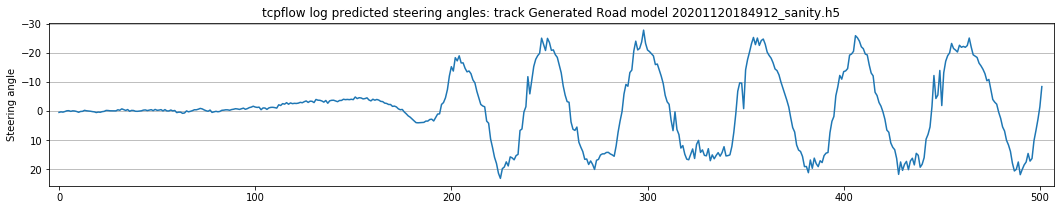
\includegraphics[width=\textwidth]{Figures/tcpflow_20201120184912_sanity_graph.png}
 \caption{Graph of steering angles recovered from tcpflow log genRoad/tcpflow/20201120184912\_sanity\_tcpflow.log for model 20201120184912\_sanity.h5 driving on Generated Road}
 \label{fig:tcpflow_20201120184912_graph}
\end{figure}

\begin{figure}[ht]
 \centering 
 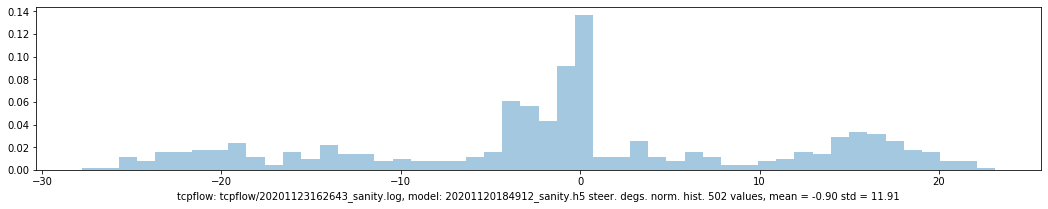
\includegraphics[width=\textwidth]{Figures/tcpflow_20201120184912_sanity_bins.png}
 \caption{Normalized histogram of tcpflow log genRoad/tcpflow/20201120184912\_ sanity \_ tcpflow.log for model 20201120184912\_ sanity.log driving on Generated Road}
 \label{fig:tcpflow_20201120184912_bins} 
\end{figure}

%%%%%%%%%%%%%%%%%%%%%%%%%%%%%%%%%%%%%%%%%%%%%%%%%%%%%%%%%%%%%%%%%%%%%%%%%%%%%
% RUN 38
%%%%%%%%%%%%%%%%%%%%%%%%%%%%%%%%%%%%%%%%%%%%%%%%%%%%%%%%%%%%%%%%%%%%%%%%%%%%%

\subsection{Run 38 - 20201123162643\_sanity.h5}
\begin{verbatim}
Commit: 1ad187d4bff5b6936c065a1aaa15a654ef4d368c
Model: nvidia1
Outputs: 2
Dataset: genRoad (clean - logs_Thu_Jul__9_16_00_15_2020 quarantined)
Command: python train.py --model=sanity --outdir=../trained\_models --epochs=5
NB Trained for 5 epochs
Environment: simbox
Comment: Rerunning commit 1ad187d4bf with cleaned data.
$ git checkout nov7 (this branch is commit 1ad187d4bff5b6936c065a1aaa15a654ef4d368c)
NB a simlink was created in unity/log2 pointing to unity/genRoad for the sake of
not changing committed source code.
ln -s ~/git/msc-data/unity/genRoad/ ~/git/msc-data/unity/log2

Epoch 1/5
1616/1616 [==============================] - 689s 427ms/step - loss: 0.0254 
- acc: 0.8033 - val_loss: 0.0167 - val_acc: 0.8365
Epoch 2/5
1616/1616 [==============================] - 681s 421ms/step - loss: 0.0186 
- acc: 0.8251 - val_loss: 0.0148 - val_acc: 0.8411
Epoch 3/5
1616/1616 [==============================] - 634s 393ms/step - loss: 0.0170 
- acc: 0.8288 - val_loss: 0.0139 - val_acc: 0.8428
Epoch 4/5
1616/1616 [==============================] - 635s 393ms/step - loss: 0.0161 
- acc: 0.8327 - val_loss: 0.0129 - val_acc: 0.8505
Epoch 5/5
1616/1616 [==============================] - 665s 411ms/step - loss: 0.0154 
- acc: 0.8365 - val_loss: 0.0125 - val_acc: 0.8451

$ cat ../trained_models/sanity/20201123162643_sanity.log
Model name: ../trained_models/sanity/20201123162643_sanity.h5
Total training time: 0:55:10
Training loss: 0.015
Validation loss: 0.013
Training accuracy: 0.836
Validation accuracy: 0.845

The batch size used by generator function was 64:
src(nov7)$ cat train.py | grep batch
def generator(samples, is_training, batch_size=64):

Running the predictions:

$ sudo tcpflow -i lo -c port 9091 > /tmp/tcpflow.log
$ python predict_client.py --model=../trained_models/sanity/20201123162643\_sanity.h5
$ python MakeVideo.py --filename=/tmp/tcpflow.log --model=20201123162643\_sanity.h5
Video uploaded to https://youtu.be/uG2HvAbg2U4

tcpflow log file moved:
cp /tmp/tcpflow.log ../dataset/unity/genRoad/tcpflow/20201123162643_sanity.log

Plotting the bins with GetSteeringAnglesFromtcpflow.ipynb

sa = GetSteeringFromtcpflow('../dataset/unity/genRoad/tcpflow/20201123162643_sanity.log')
sarr = np.asarray(sa)
p = sarr[:,0]
p = sarr[:,0]  
plotSteeringAngles(p, g, 25, False, "Generated Road", "20201123162643_sanity.h5")
plotBinsFromArray(p, 25, "20201123162643_sanity.h5", "tcpflow/20201123162643_sanity.log") 
\end{verbatim}

Steering data recovered from tcpflow log genRoad/tcpflow/20201123162643\_sanity.log
This was running with commit 1ad187d4bf where frame \textbf{is not preprocessed} for prediction (predict\_ client.py) (Figures  \ref{fig:tcpflow_20201123162643_graph} and  \ref{fig:tcpflow_20201123162643_bins}). 

\begin{figure}[ht]
 \centering 
 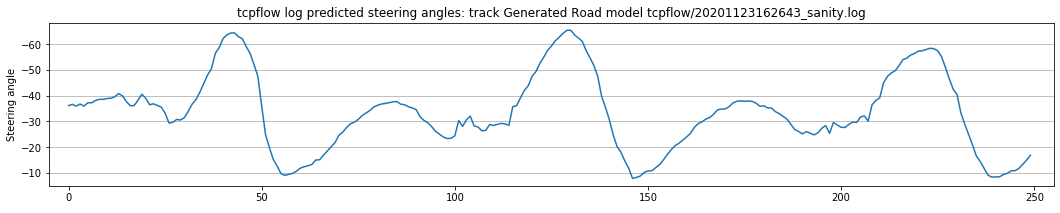
\includegraphics[width=\textwidth]{Figures/tcpflow_20201123162643_sanity_graph.png}
 \caption{Graph of steering angles recovered from tcpflow log genRoad/tcpflow/20201123162643\_sanity.log for model 20201123162643\_sanity.h5 driving on Generated Road}. The video can be seen here \href{https://youtu.be/uG2HvAbg2U4}{https://youtu.be/uG2HvAbg2U4}
 \label{fig:tcpflow_20201123162643_graph}
\end{figure}

\begin{figure}[ht]
 \centering 
 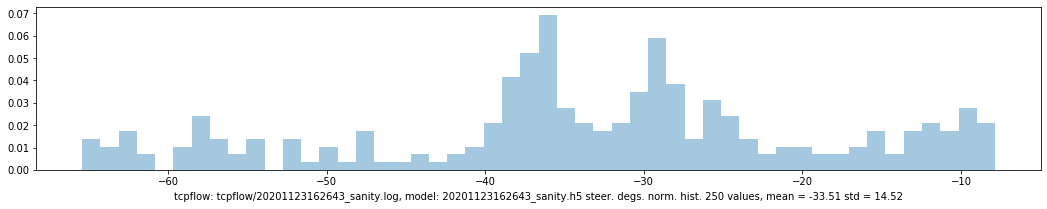
\includegraphics[width=\textwidth]{Figures/tcpflow_20201123162643_sanity_bins.png}
 \caption{Normalized histogram of tcpflow log genRoad/tcpflow/20201123162643\_ sanity.log for model 20201123162643\_ sanity.log driving on Generated Road}
 \label{fig:tcpflow_20201123162643_bins} 
\end{figure} 

%%%%%%%%%%%%%%%%%%%%%%%%%%%%%%%%%%%%%%%%%%%%%%%%%%%%%%%%%%%%%%%%%%%%%%%%%%%%%
% RUN 39
%%%%%%%%%%%%%%%%%%%%%%%%%%%%%%%%%%%%%%%%%%%%%%%%%%%%%%%%%%%%%%%%%%%%%%%%%%%%%
\subsection{Run 39 - 20201123162643\_sanity.h5}
\begin{verbatim}
Commit: 7f3086490118fec1a20e99e93cc1b853a91272b6
Model:  N/A (trained model)
Outputs:N/A (trained model)
Dataset: N/A (trained model)
Command: 
Environment: 
Comment: Same as previous run, but on branch 7f308649 (predict_client.py) with
preprocessing

$ sudo tcpflow -i lo -c port 9091 (right angle bracket) /tmp/tcpflow.log
$ python predict_client.py
--model=../trained_models/sanity/20201123162643\_sanity.h5
$ python MakeVideo.py --filename=/tmp/tcpflow.log --model=20201123162643\_sanity.h5

Link: https://youtu.be/377O2E_LwyU

tcpflow log file moved:
cp /tmp/tcpflow.log ../dataset/unity/genRoad/tcpflow/20201123162643_sanity_pp.log

sa = GetSteeringFromtcpflow('../dataset/unity/genRoad/tcpflow/20201123162643_
sanity_pp.log')
sarr = np.asarray(sa)
p = sarr[:,0]
p = sarr[:,0]  
plotSteeringAngles(p, g, 25, False, "Generated Road", "20201123162643
_sanity_pp.h5")
plotBinsFromArray(p, 25, "20201123162643_sanity.h5",
"tcpflow/20201123162643_sanity_pp.log")

Video: https://youtu.be/377O2E_LwyU
\end{verbatim}

Steering data recovered from tcpflow log genRoad/tcpflow/20201123162643\_sanity\_pp.log
This was running with commit 7f308649 where frame \textbf{is preprocessed} for prediction (predict\_ client.py) (Figures  \ref{fig:tcpflow_20201123162643_pp_graph} and  \ref{fig:tcpflow_20201123162643_pp_bins}). 
Note the steering angles are a much tighter range. Bias toward positive 6 is due to road bending right.
The bins show a left skewed distribution, due to the right turn. Steering goes a bit crazy but model
manages to keep vehicle on the road.

\begin{figure}[ht]
 \centering 
 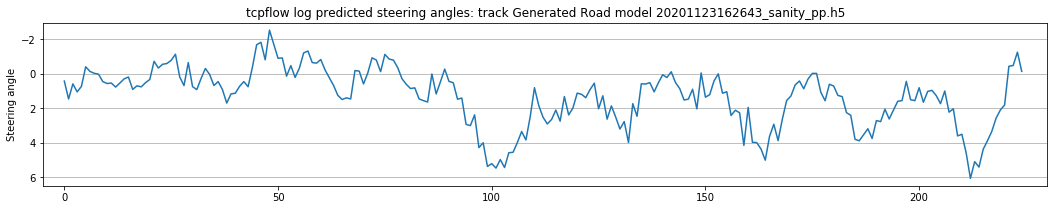
\includegraphics[width=\textwidth]{Figures/tcpflow_20201123162643_sanity_pp_graph.png}
 \caption{Graph of steering angles recovered from tcpflow log genRoad/tcpflow/20201123162643\_ sanity\_  pp.log for model 20201123162643\_ sanity.h5 driving on Generated Road}. The video can be seen here \href{https://youtu.be/377O2E\_ LwyU}{https://youtu.be/377O2E\_ LwyU}
 \label{fig:tcpflow_20201123162643_pp_graph}
\end{figure}

\begin{figure}[ht]
 \centering 
 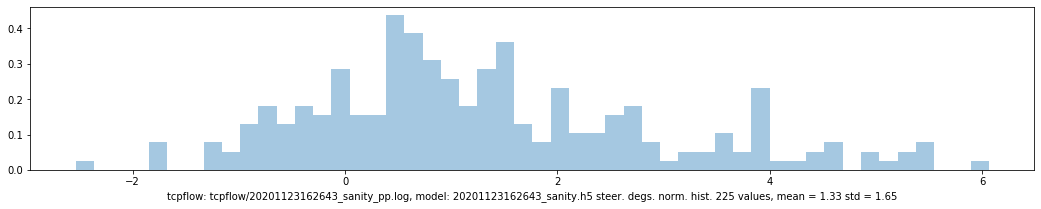
\includegraphics[width=\textwidth]{Figures/tcpflow_20201123162643_sanity_pp_bins.png}
 \caption{Normalized histogram of tcpflow log genRoad/tcpflow/20201123162643\_ sanity\_ pp.log for model 20201123162643\_sanity.h5 driving on Generated Road}
 \label{fig:tcpflow_20201123162643_pp_bins} 
\end{figure} 

%%%%%%%%%%%%%%%%%%%%%%%%%%%%%%%%%%%%%%%%%%%%%%%%%%%%%%%%%%%%%%%%%%%%%%%%%%%%%
% RUN 40
%%%%%%%%%%%%%%%%%%%%%%%%%%%%%%%%%%%%%%%%%%%%%%%%%%%%%%%%%%%%%%%%%%%%%%%%%%%%%
\subsection{Run 40 - 20201124032017\_ nvidia2.h5}
\begin{verbatim}
Commit: 7f3086490118fec1a20e99e93cc1b853a91272b6
Model: nvidia1
Outputs: 2
Dataset: N/A
Command: python3 train.py --model=nvidia2 --outdir=../trained_models --epochs=100
Environment: devcloud
Comment: Trained with nvidia2 model. Need to double check input size, as it might
be originally expecting 200x66.
Model did not do well and drove straight off the road. One thing to note, pixels are
being normalized and zero centered:
x = Lambda(lambda x: x/127.5 - 1.0)
Also, one single dropout layer. Need to try with different image size to match
original design.

$ sudo tcpflow -i lo -c port 9091 (right angle bracket) /tmp/tcpflow.log
$ python predict_client.py
--model=../trained_models/devcloud/nvidia2/20201124032017_nvidia2.h5
$ python MakeVideo.py --filename=/tmp/tcpflow.log --model=20201124032017\_nvidia2.h5

https://youtu.be/RW-luOWQ_qY

tcpflow log file moved:
cp /tmp/tcpflow.log ../dataset/unity/genRoad/tcpflow/20201124032017_nvidia2.log

sa = GetSteeringFromtcpflow('../dataset/unity/genRoad/tcpflow/20201124032017_nvidia2.log)
sarr = np.asarray(sa)
p = sarr[:,0]
p = sarr[:,0]  
plotSteeringAngles(p, g, 25, False, "Generated Road", "20201124032017_nvidia2.h5")
plotBinsFromArray(p, 25, "20201124032017_nvidia2.h5", "tcpflow/20201124032017_nvidia2.log")
\end{verbatim}

Run 40 started well then pretty much drove straight off the road - need to investigate image
geometry
\begin{figure}[ht]
 \centering 
 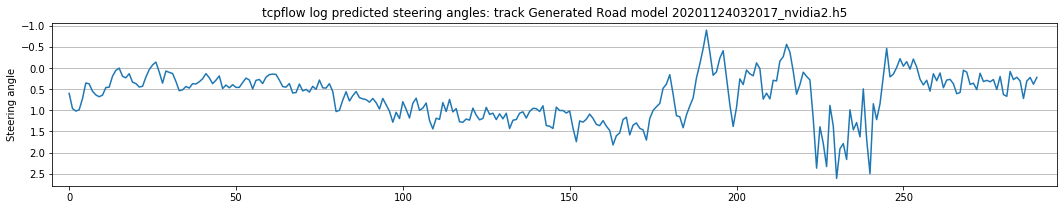
\includegraphics[width=\textwidth]{Figures/tcpflow_20201124032017_nvidia2_graph.png}
 \caption{Graph of steering angles recovered from tcpflow log genRoad/tcpflow/20201124032017\_ nvidia2.log for model 20201124032017\_ nvidia2.h5 driving on Generated Road}. The video can be seen here \href{https://youtu.be/RW-luOWQ\_ qY}{https://youtu.be/RW-luOWQ\_ qY}
 \label{fig:tcpflow_20201124032017_nvidia2_graph}
\end{figure}

\begin{figure}[ht]
 \centering 
 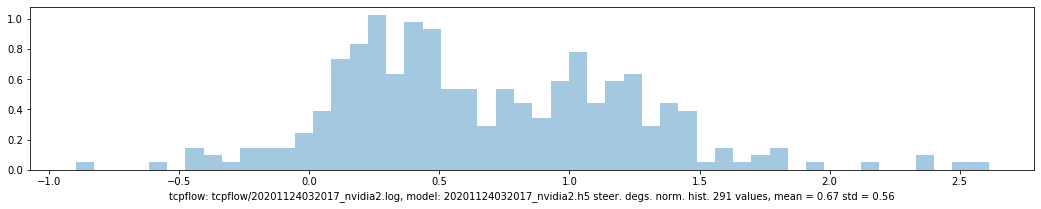
\includegraphics[width=\textwidth]{Figures/tcpflow_20201124032017_nvidia2_bins.png}
 \caption{Normalized histogram of tcpflow log genRoad/tcpflow/20201124032017\_ nvidia2.log for model 20201124032017\_ nvidia2.h5 driving on Generated Road}
 \label{fig:tcpflow_20201124032017_nvidia2_bins} 
\end{figure} 


%%%%%%%%%%%%%%%%%%%%%%%%%%%%%%%%%%%%%%%%%%%%%%%%%%%%%%%%%%%%%%%%%%%%%%%%%%%%%
% RUN 41
%%%%%%%%%%%%%%%%%%%%%%%%%%%%%%%%%%%%%%%%%%%%%%%%%%%%%%%%%%%%%%%%%%%%%%%%%%%%%
\subsection{Run 41 - 20201120171015\_ sanity.h5}
\label{app_res:41}
\label{}
\begin{verbatim}
Commit: f0d2513
Model: nvidia1
Outputs: 2
Dataset: log_sample (small looping circuit)

Command: 

$ sudo tcpflow -i lo -c port 9091 > /tmp/tcpflow_20201120171015_sanity.log
$ python predict_client.py --model=../trained_models/sanity/20201120171015_sanity.h5
$ python MakeVideo.py --filename=/tmp/tcpflow_20201120171015_sanity.log
--model=20201120171015_sanity.h5
# mv
$ mv /tmp/tcpflow_20201120171015_sanity.log \ 
~/git/sdsandbox/trained_models/sanity/tcpflow/

Generating plot:
$ python steerlib.py
$ python 
>>> import steerlib as sl
>>> sa = sl.etSteeringFromtcpflow('../../dataset/unity/genRoad/tcpflow/tcpflow_20201
120171015_sanity.log')
>>> sarr = np.asarray(sa)
>>> p = sarr[:,0]

plot = sl.plotSteeringAngles(p, None, 25, True, "Generated Track",
"20201120171015_sanity.h5", 'tcpflow log predicted')
Environment: simbox
Comment: Prediction to generate tcpflow log
video https://youtu.be/LEmZJJzJkEE
\end{verbatim}

%%%%%%%%%%%%%%%%%%%%%%%%%%%%%%%%%%%%%%%%%%%%%%%%%%%%%%%%%%%%%%%%%%%%%%%%%%%%%
% RUN 42
%%%%%%%%%%%%%%%%%%%%%%%%%%%%%%%%%%%%%%%%%%%%%%%%%%%%%%%%%%%%%%%%%%%%%%%%%%%%%
\subsection{Run 42 - 20201120171015\_ sanity.h5}
\label{app_res:42}
\begin{verbatim}
Commit: 444c27f 
Model: Outputs: Dataset: Command: Environment: Same as run 41 
Comment: Testing conversion of PIL image to numpy array, bypassing saving .jpg to
disk and reading from disk.

git diff ef4b48e..444c27f1 MakeVideo.py
diff --git a/src/utils/MakeVideo.py b/src/utils/MakeVideo.py
index f469471..8abd3c8 100644
--- a/src/utils/MakeVideo.py
+++ b/src/utils/MakeVideo.py
(...)
                     image = Image.open(BytesIO(base64.b64decode(imgString)))
+                    # try to convert to jpg
+                    image = np.array(image)
(...)



\end{verbatim}

Video still (Figure \ref{fig:tcpflow_Run42}) showing effect of converting PIL image directly to numpy array. Colour of sky is different.
No video was uploaded to youtube.


\begin{figure}[h!]
\centering
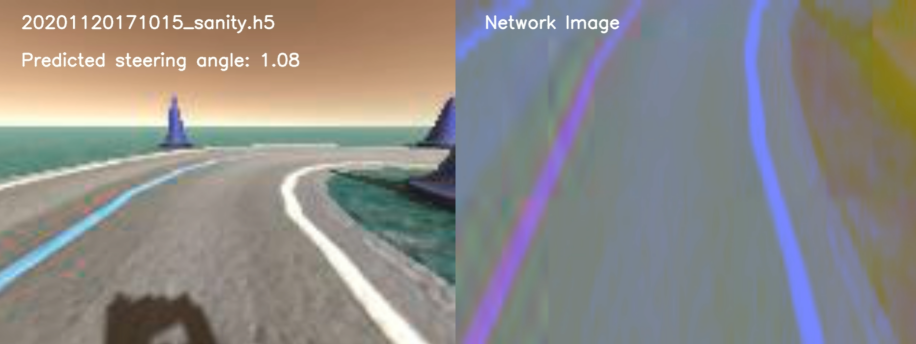
\includegraphics[width=\textwidth]{Figures/tcpflow_Run42.png}
\caption{tcpflow log image converted directly to numpy array (left) and image presented to network (right).}
\label{fig:tcpflow_Run42}
\end{figure}




%%%%%%%%%%%%%%%%%%%%%%%%%%%%%%%%%%%%%%%%%%%%%%%%%%%%%%%%%%%%%%%%%%%%%%%%%%%%%
% RUN 43
%%%%%%%%%%%%%%%%%%%%%%%%%%%%%%%%%%%%%%%%%%%%%%%%%%%%%%%%%%%%%%%%%%%%%%%%%%%%%
\subsection{Run 43 - Record triple video}
On this run we record a video with 3 frames side by side containing the simulator image, simulator image with added rain and the preprocessed image with added rain.

Interesting observation here (pending two tests to be documented), when we change the order of added rain, i.e. added to image before preprocesssing or added to image after preprocessing, this affects the outcome. Conclusion is currently pointing to the fact that moving image space from RGB to YUV is filtering out the rain "noise"

\label{app_res:43}
\begin{verbatim}
Commit: b0a77d2
Model: Outputs: Dataset: Environment: Same as run 41 
Command: 
$ python predict_client.py --model=../trained_models/sanity/20201120171015_sanity.h5
--rain=torrential --slant=20 --record=true

Video https://youtu.be/57jwwcjbfdE

Comment: As observed if noise is added to preprocessed image (at the point of being
presented to network), sim crashes.

\end{verbatim}



%%%%%%%%%%%%%%%%%%%%%%%%%%%%%%%%%%%%%%%%%%%%%%%%%%%%%%%%%%%%%%%%%%%%%%%%%%%%%
% RUN 44
%%%%%%%%%%%%%%%%%%%%%%%%%%%%%%%%%%%%%%%%%%%%%%%%%%%%%%%%%%%%%%%%%%%%%%%%%%%%%
\subsection{Run 44 - Intensity x4}
\begin{verbatim}
Commit: 9696f3cee
Model: Outputs: Dataset: Environment: Same as run 41 
Command: 
$ python predict_client.py --model=../trained_models/sanity/20201120171015_sanity.h5 \
--rain=heavy --slant=20 --record=True

Comment: Changed luminosity multiply manually 
tcpflow file: (TODO plot steering including crash section)
~/git/sdsandbox/trained_models/sanity/tcpflow/20201120171015_sanity_run44.log

Video: https://youtu.be/UBd38Hlfv4w

\end{verbatim}


%%%%%%%%%%%%%%%%%%%%%%%%%%%%%%%%%%%%%%%%%%%%%%%%%%%%%%%%%%%%%%%%%%%%%%%%%%%%%
% RUN 45
%%%%%%%%%%%%%%%%%%%%%%%%%%%%%%%%%%%%%%%%%%%%%%%%%%%%%%%%%%%%%%%%%%%%%%%%%%%%%
\subsection{Run 45 - Intensity x8}
\begin{verbatim}
Commit: 20fe20c2e
Model: Outputs: Dataset: Environment: Same as run 41 
Command: 
$ python predict_client.py --model=../trained_models/sanity/20201120171015_sanity.h5
--rain=heavy --slant=20 --record=True
Comment: Changed intensity manually to 8, vehicle stays on road for 2 laps.
Higher intensity means higher contrast between road and non-road, perhaps creating 
a guiding pattern.
It suggests there is some generalisation, as road is very unfamiliar.

tcpflow file:
~/git/sdsandbox/trained_models/sanity/tcpflow/20201120171015_sanity_run45.log

Video https://youtu.be/NerkRCSquiE
\end{verbatim}


%%%%%%%%%%%%%%%%%%%%%%%%%%%%%%%%%%%%%%%%%%%%%%%%%%%%%%%%%%%%%%%%%%%%%%%%%%%%%
% RUN 46
%%%%%%%%%%%%%%%%%%%%%%%%%%%%%%%%%%%%%%%%%%%%%%%%%%%%%%%%%%%%%%%%%%%%%%%%%%%%%
\subsection{Run 46 - 20201203164029\_ nvidia1.h5}
%\label{app_res:46}
\begin{verbatim}
Commit: 2d9e6983
Model: N/A
Outputs: N/A
Dataset: genTrack
Command: 
$ python train.py --model=nvidia1 --outdir=../trained_models --epochs=100
--inputs=../dataset/genTrackOneLap/*.jpg --aug=true --preproc=true
--inputs=../dataset/unity/genTrack/*.jpg
Environment: devbox
Comment: Gathered dataset (35967 files) moved to ../dataset/unity/genTrack
ls -R | grep .jpg | wc -l
35967
Laps recorded with settings:
Max Speed 1.963599
Prop: 24
Diff: 5
Steer Max: 25
\end{verbatim}

%%%%%%%%%%%%%%%%%%%%%%%%%%%%%%%%%%%%%%%%%%%%%%%%%%%%%%%%%%%%%%%%%%%%%%%%%%%%%
% RUN 47
%%%%%%%%%%%%%%%%%%%%%%%%%%%%%%%%%%%%%%%%%%%%%%%%%%%%%%%%%%%%%%%%%%%%%%%%%%%%%
\subsection{Run 47 - 20201206171648\_ nvidia1.h5}
%\label{app_res:47}
\begin{verbatim}
Commit: 3f0622c8
Model: nvidia1
Outputs: 2
Dataset: genRoad
Command: python train.py
--model=nvidia1
--outdir=../trained_models
--epochs=5
--inputs=../dataset/unity/genRoad/*.jpg
--aug=True
--preproc=True
Environment: simbox
Comment: Created Augmentation class, handling image sizes for different models.
Then ran:
python predict_client.py --model=../trained_models/nvidia1/20201206171648_nvidia1.h5

When running this model (and possibly all previous):

$ python predict_client.py --model=../trained_models/nvidia1/20201206171648_nvidia1.h5

WARNING:tensorflow:Model was constructed with shape (None, 160, 120, 3) for input
Tensor("img_in:0", shape=(None, 160, 120, 3), dtype=float32), but it was called on
an input with incompatible shape (None, 120, 160, 3).

As it turns out, it was an assignment mess up. See diff on models.py between runs 
48 and 49.

Still the "flipped" input model did manage a stretch of Generated Road and
surprisingly manages to get around Generated Track, which is a total fluke, which
may prove serendipitous.

TODO ADD TO DISCUSSION (TOTAL FLUKE FLIP)
\end{verbatim}


%%%%%%%%%%%%%%%%%%%%%%%%%%%%%%%%%%%%%%%%%%%%%%%%%%%%%%%%%%%%%%%%%%%%%%%%%%%%%
% RUN 48
%%%%%%%%%%%%%%%%%%%%%%%%%%%%%%%%%%%%%%%%%%%%%%%%%%%%%%%%%%%%%%%%%%%%%%%%%%%%%
\subsection{Run 48 - 20201206211122\_ nvidia1.h5}
%\label{app_res:48}
\begin{verbatim}
Commit: b5ad97f
Model: nvidia1
Outputs: 2
Dataset: genRoad
Command: python train.py
--model=nvidia1
--outdir=../trained_models
--epochs=5
--inputs=../dataset/unity/genRoad/*.jpg
--aug=True
--preproc=True
Environment: simbox
Comment: Based on previous (Run 47 warning), input to network was changed to col, row,
channels. NB This was an oversight. In the next run, col, row remain, the assignment
changes (to fix mix-up).

This model did really well on Generated Road but not well at all on Generated Track.
\end{verbatim}

%%%%%%%%%%%%%%%%%%%%%%%%%%%%%%%%%%%%%%%%%%%%%%%%%%%%%%%%%%%%%%%%%%%%%%%%%%%%%
% RUN 49 - PROBABLY BEST NVIDIA1 MODEL
%%%%%%%%%%%%%%%%%%%%%%%%%%%%%%%%%%%%%%%%%%%%%%%%%%%%%%%%%%%%%%%%%%%%%%%%%%%%%
\subsection{Run 49 - 20201207091932\_ nvidia1.h5}
\label{app_res:49}
\begin{verbatim}
Commit: 55cb00b
Model: nvidia1
Outputs: 2
Dataset: genTrack
Command: 
$ python train.py
--model=nvidia1
--outdir=../trained_models
--epochs=5
--inputs=../dataset/unity/genTrack/*.jpg
--aug=True
--preproc=True

Environment: simbox
Comment: Trained for 5 epochs, maximum validation accuracy 0.7644. This model
drives both on Generated Road and Generated Track. This model took 1m23s to
train.

$ cat ../trained_models/nvidia1/20201207091932_nvidia1.log
Model name: ../trained_models/nvidia1/20201207091932_nvidia1.h5
Total training time: 0:01:23
Training loss: 0.021
Validation loss: 0.015
Training accuracy: 0.751
Validation accuracy: 0.757

Recording with no rain:
python predict_client.py
--model=../trained_models/nvidia1/20201207091932_nvidia1.h5 --record=True
https://youtu.be/S-PBNgJ_mdY

tcpflow log:
../trained_models/nvidia1/tcpflow/20201207091932_nvidia1_tcpflow.log

\end{verbatim}

Video of image plus network image - no rain - Generated Road:  
\url{https://youtu.be/S-PBNgJ_mdY} 

Figure \ref{fig:20201207091932_nvidia1_tcpflow} shows a slight positive value (road turning right) to start with, then a negative value (road turning left) steering angle.

\begin{figure}[ht]
 \centering 
 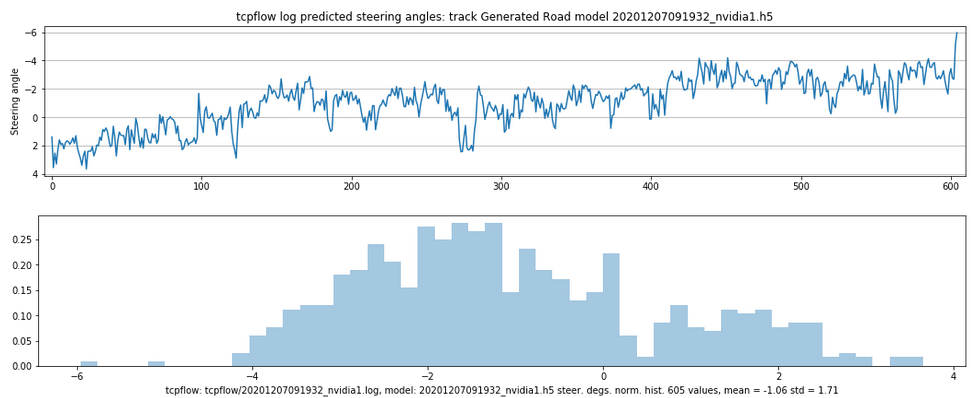
\includegraphics[width=\textwidth]{Figures/20201207091932_nvidia1_tcpflow.png}
 \caption{tcpflow steering angle log for model 20201207091932\_ nvidia1.h5 trained over 5 epochs on Generated Track, self-driving in a section of Generated Road}
 \label{fig:20201207091932_nvidia1_tcpflow}
\end{figure}

%%%%%%%%%%%%%%%%%%%%%%%%%%%%%%%%%%%%%%%%%%%%%%%%%%%%%%%%%%%%%%%%%%%%%%%%%%%%%
% RUN 50
%%%%%%%%%%%%%%%%%%%%%%%%%%%%%%%%%%%%%%%%%%%%%%%%%%%%%%%%%%%%%%%%%%%%%%%%%%%%%
\subsection{Run 50 - 20201207111940\_ nvidia2.h5}
%\label{app_res:50}
\begin{verbatim}
Commit: f9325ff
Model: nvidia2
Outputs: 2
Dataset: genTrack
Command: python train.py
--model=nvidia2
--outdir=../trained_models
--epochs=5
--inputs=../dataset/unity/genTrack/*.jpg
--aug=True
--preproc=True

Environment: simbox
Comment: Model trained with 0.5 dropout in a single layer. nvidia1 is trained
with 5 dropout layers at 0.1 each.

Running the model:
$ cd ~/Downloads
$ ./startunity.sh
$ sudo tcpflow -i lo -c port 9091 > /tmp/tcpflow.log
python predict_client.py
--model=../trained_models/nvidia2/20201207111940_nvidia2.h5
--modelname=nvidia2
--record=True

Video: https://youtu.be/b6IIoHuiUQ8

\end{verbatim}

Figure \ref{fig:20201207111940_nvidia2_tcpflow} shows a tcpflow of the nvidia2 model driving off the road by over-steering to the left after the first right turn as can be seen in video \url{https://youtu.be/b6IIoHuiUQ8} 

\begin{figure}[ht]
 \centering 
 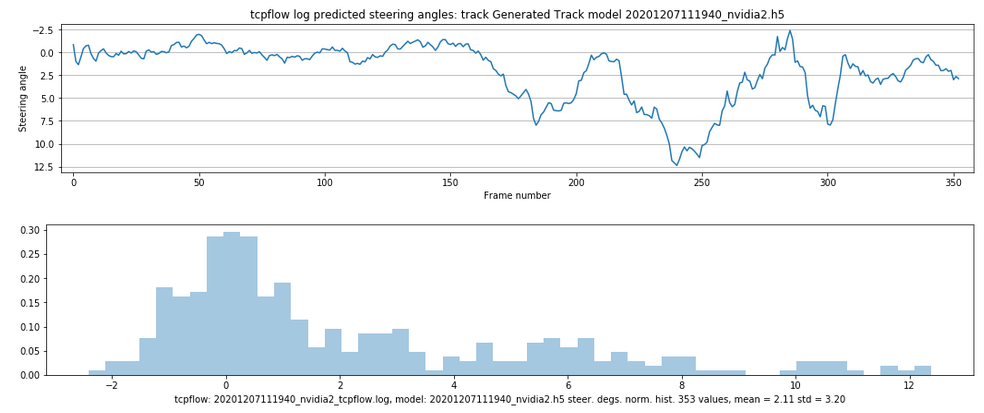
\includegraphics[width=\textwidth]{Figures/20201207111940_nvidia2_tcpflow.png}
 \caption{tcpflow steering angle log for model 20201207111940\_ nvidia2.h5 trained over 5 epochs on Generated Roard, self-driving off the road after first right turn.}
 \label{fig:20201207111940_nvidia2_tcpflow}
\end{figure}

%%%%%%%%%%%%%%%%%%%%%%%%%%%%%%%%%%%%%%%%%%%%%%%%%%%%%%%%%%%%%%%%%%%%%%%%%%%%%
% RUN 51
%%%%%%%%%%%%%%%%%%%%%%%%%%%%%%%%%%%%%%%%%%%%%%%%%%%%%%%%%%%%%%%%%%%%%%%%%%%%%
\subsection{Run 51 - 20201207124146\_ nvidia2.h5 }
%\label{app_res:51}
\begin{verbatim}
Commit: bb66ed7
Comment: Same as run 50, with dropout set to 0.25

$ python predict_client.py --model=../trained_models/nvidia2/20201207124146_nvidia2.h5
--modelname=nvidia2 --record=True

Video: https://youtu.be/-lDaiodokxw

\end{verbatim}

Figure \ref{fig:20201207124146_nvidia2_tcpflow} shows a tcpflow log of the nvidia2 model driving off the road by over-steering to the left off the first right turn as can be seen in video \url{https://youtu.be/-lDaiodokxw}. The model was trained with a single 0.25 dropout layer

\begin{figure}[ht]
 \centering 
 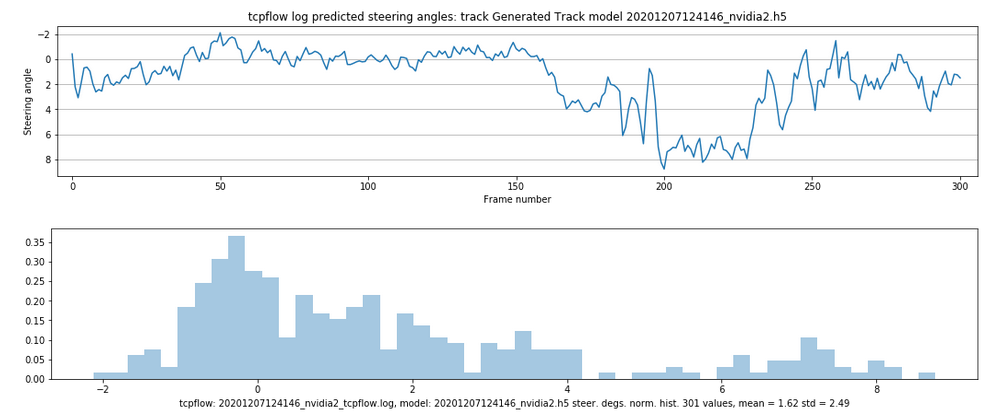
\includegraphics[width=\textwidth]{Figures/20201207124146_nvidia2_tcpflow.png}
 \caption{tcpflow steering angle log for model 20201207124146\_ nvidia2.h5 trained over 5 epochs on Generated Track, with droupout set to 0.25, self-driving off the road after first right turn.}
 \label{fig:20201207124146_nvidia2_tcpflow}
\end{figure}


%%%%%%%%%%%%%%%%%%%%%%%%%%%%%%%%%%%%%%%%%%%%%%%%%%%%%%%%%%%%%%%%%%%%%%%%%%%%%
% RUN 52
%%%%%%%%%%%%%%%%%%%%%%%%%%%%%%%%%%%%%%%%%%%%%%%%%%%%%%%%%%%%%%%%%%%%%%%%%%%%%
\subsection{Run 52 - 20201207132429\_ nvidia2.h5}
\label{app_res:52}
\begin{verbatim}
Commit: cd3aa3a
Comment: Same as 51, with dropout set to 0.1

$ python predict_client.py 
--model=../trained_models/nvidia2/20201207132429_nvidia2.h5 
--modelname=nvidia2 --record=True

https://youtu.be/I6aB5RxYPsg

\end{verbatim}

Another case where nvidia2 drives off the road on the first right turn (Figure \ref{fig:20201207132429_nvidia2_tcpflow}). \url{https://youtu.be/I6aB5RxYPsg}.
\begin{figure}[ht]
 \centering 
 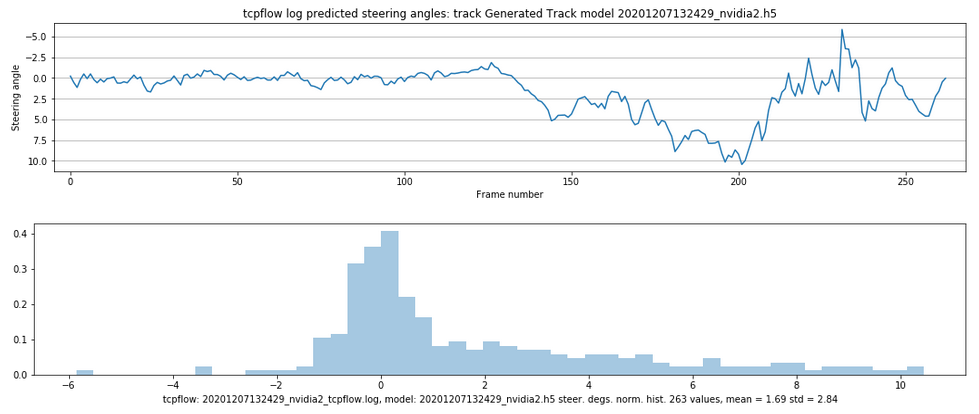
\includegraphics[width=\textwidth]{Figures/20201207132429_nvidia2_tcpflow.png}
 \caption{tcpflow steering angle log for model 220201207132429\_ nvidia2.h5 trained over 5 epochs on Generated Road, with dropout set to 0.1, self-driving off the road after first right turn.}
 \label{fig:20201207132429_nvidia2_tcpflow}
\end{figure}

%%%%%%%%%%%%%%%%%%%%%%%%%%%%%%%%%%%%%%%%%%%%%%%%%%%%%%%%%%%%%%%%%%%%%%%%%%%%%
% RUN 53
%%%%%%%%%%%%%%%%%%%%%%%%%%%%%%%%%%%%%%%%%%%%%%%%%%%%%%%%%%%%%%%%%%%%%%%%%%%%%
\subsection{Run 53 - 20201207133600\_ nvidia2.h5 }
%\label{app_res:XX}
\begin{verbatim}
Commit: 3e3ff1a
Comment: Same as 52 except last dense layer (10 units) removed
$ git diff --name-only cd3aa3a..3e3ff1a
src/GetSteeringAnglesFromtcpflow.ipynb
src/models.py

$ git diff cd3aa3a..3e3ff1a models.py
diff --git a/src/models.py b/src/models.py
index 0ef889e..8efe891 100644
--- a/src/models.py
+++ b/src/models.py
@@ -165,7 +165,7 @@ def nvidia_model2(num_outputs):
     # x = Dropout(drop)(x)
     x = Dense(50, activation='elu')(x)
     # x = Dropout(drop)(x)
-    x = Dense(10, activation='elu')(x) # Added in Naoki's model
+    # x = Dense(10, activation='elu')(x) # Added in Naoki's model

\end{verbatim}

Slightly better but still drives off road past the second left bollard.

The model:
\begin{verbatim}
_________________________________________________________________
Layer (type)                 Output Shape              Param #   
=================================================================
img_in (InputLayer)          [(None, 66, 200, 3)]      0         
_________________________________________________________________
lambda (Lambda)              (None, 66, 200, 3)        0         
_________________________________________________________________
conv2d_1 (Conv2D)            (None, 31, 98, 24)        1824      
_________________________________________________________________
conv2d_2 (Conv2D)            (None, 14, 47, 36)        21636     
_________________________________________________________________
conv2d_3 (Conv2D)            (None, 5, 22, 48)         43248     
_________________________________________________________________
conv2d_4 (Conv2D)            (None, 3, 20, 64)         27712     
_________________________________________________________________
conv2d_5 (Conv2D)            (None, 1, 18, 64)         36928     
_________________________________________________________________
dropout (Dropout)            (None, 1, 18, 64)         0         
_________________________________________________________________
flattened (Flatten)          (None, 1152)              0         
_________________________________________________________________
dense (Dense)                (None, 100)               115300    
_________________________________________________________________
dense_1 (Dense)              (None, 50)                5050      
_________________________________________________________________
steering_throttle (Dense)    (None, 2)                 102       
=================================================================
Total params: 251,800
Trainable params: 251,800
Non-trainable params: 0
_________________________________________________________________
[(None, 66, 200, 3)]    
\end{verbatim}

Video: \url{https://youtu.be/DPxFLukN0Ws}

%%%%%%%%%%%%%%%%%%%%%%%%%%%%%%%%%%%%%%%%%%%%%%%%%%%%%%%%%%%%%%%%%%%%%%%%%%%%%
% RUN 54
%%%%%%%%%%%%%%%%%%%%%%%%%%%%%%%%%%%%%%%%%%%%%%%%%%%%%%%%%%%%%%%%%%%%%%%%%%%%%
\subsection{Run 54 - 20201207141017\_ nvidia2.h5}
%\label{app_res:54}
\begin{verbatim}
Commit: a39008c
Comment: Same as run 53 except dropout layers added as per nvidia1. Note
zero-centered pixel values in git diff below:

$ git diff 3e3ff1a..a39008c models.py
diff --git a/src/models.py b/src/models.py
index 8efe891..28e6d62 100644
--- a/src/models.py
+++ b/src/models.py
@@ -149,13 +149,13 @@ def nvidia_model2(num_outputs):
     x = Lambda(lambda x: x/127.5 - 1.0)(x) # normalize and re-center
     # x = Lambda(lambda x: x / 255.0)(x)
     x = Conv2D(24, (5, 5), strides=(2, 2), activation='elu', name="conv2d_1")(x)
-    # x = Dropout(drop)(x)
+    x = Dropout(drop)(x)
     x = Conv2D(36, (5, 5), strides=(2, 2), activation='elu', name="conv2d_2")(x)
-    #x = Dropout(drop)(x)
+    x = Dropout(drop)(x)
     x = Conv2D(48, (5, 5), strides=(2, 2), activation='elu', name="conv2d_3")(x)
-    #x = Dropout(drop)(x)
+    x = Dropout(drop)(x)
     x = Conv2D(64, (3, 3), activation='elu', name="conv2d_4")(x) # default strides=(1,1)
-    #x = Dropout(drop)(x)
+    x = Dropout(drop)(x)
     x = Conv2D(64, (3, 3), activation='elu', name="conv2d_5")(x)
     x = Dropout(drop)(x)

Veers off road a little bit after run 53.
\end{verbatim}
Video: \url{https://youtu.be/SQQJacV622E}

Network:
\begin{verbatim}
import models
mymodel = models.nvidia_model2(2)
models.show_model_summary(mymodel)
Model: "model_1"
Layer (type)                 Output Shape              Param #   
=================================================================
img_in (InputLayer)          [(None, 66, 200, 3)]      0         
_________________________________________________________________
lambda (Lambda)              (None, 66, 200, 3)        0         
_________________________________________________________________
conv2d_1 (Conv2D)            (None, 31, 98, 24)        1824      
_________________________________________________________________
dropout (Dropout)            (None, 31, 98, 24)        0         
_________________________________________________________________
conv2d_2 (Conv2D)            (None, 14, 47, 36)        21636     
_________________________________________________________________
dropout_1 (Dropout)          (None, 14, 47, 36)        0         
_________________________________________________________________
conv2d_3 (Conv2D)            (None, 5, 22, 48)         43248     
_________________________________________________________________
dropout_2 (Dropout)          (None, 5, 22, 48)         0         
_________________________________________________________________
conv2d_4 (Conv2D)            (None, 3, 20, 64)         27712     
_________________________________________________________________
dropout_3 (Dropout)          (None, 3, 20, 64)         0         
_________________________________________________________________
conv2d_5 (Conv2D)            (None, 1, 18, 64)         36928     
_________________________________________________________________
dropout_4 (Dropout)          (None, 1, 18, 64)         0         
_________________________________________________________________
flattened (Flatten)          (None, 1152)              0         
_________________________________________________________________
dense (Dense)                (None, 100)               115300    
_________________________________________________________________
dense_1 (Dense)              (None, 50)                5050      
_________________________________________________________________
steering_throttle (Dense)    (None, 2)                 102       
=================================================================
Total params: 251,800
Trainable params: 251,800
Non-trainable params: 0
_________________________________________________________________
[(None, 66, 200, 3)]
(None, 66, 200, 3)
(None, 31, 98, 24)
(None, 31, 98, 24)
(None, 14, 47, 36)
(None, 14, 47, 36)
(None, 5, 22, 48)
(None, 5, 22, 48)
(None, 3, 20, 64)
(None, 3, 20, 64)
(None, 1, 18, 64)
(None, 1, 18, 64)
(None, 1152)
(None, 100)
(None, 50)
(None, 2)

\end{verbatim}

%%%%%%%%%%%%%%%%%%%%%%%%%%%%%%%%%%%%%%%%%%%%%%%%%%%%%%%%%%%%%%%%%%%%%%%%%%%%%
% RUN 55
%%%%%%%%%%%%%%%%%%%%%%%%%%%%%%%%%%%%%%%%%%%%%%%%%%%%%%%%%%%%%%%%%%%%%%%%%%%%%
\subsection{Run 55 - 20201207142129\_ nvidia2.h5}
%\label{app_res:55}
\begin{verbatim}
Commit: 28ea337
Comment: Same as 54, except aligned number of nvidia2 feature maps with nvidia1
\end{verbatim}
Another crash (\url{https://youtu.be/3ipZZgGtJUA}). Given that nvidia1 () run 52 did so well and every subsequent nvidia2 has crashed. Let's have a look at the actual crop we are presenting to both networks (Figure \ref{fig:2129x1932crops}):
 
\begin{figure}[ht]
 \centering 
 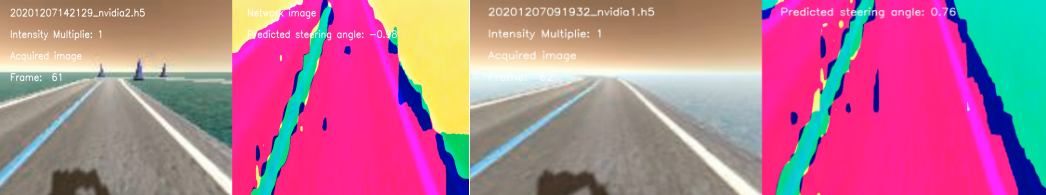
\includegraphics[width=\textwidth]{Figures/2129x1932crops.png}
 \caption{Network images presented to networks nvidia2 (20201207142129\_ nvidia2.h5) network (second from left) and nvidia1 (20201207091932\_ nvidia1.h5), first on right}
 \label{fig:2129x1932crops}
\end{figure}

What is most noticeable is that the nvidia1 network image seems to somehow augment the road information, by making it cover more of the image.
If we look at the actual dimension crops up to commit 28ea337 on master branch, in conf.py:
\begin{verbatim}
# NVIDIA1
NVIDIA1 = 'nvidia1' # a.k.a. TawnNet
nvidia1_img_dims = [160,120,3,160,120,60,-25]
# NVIDIA2
NVIDIA2 = 'nvidia2' # a.k.a. NaokiNet
nvidia2_img_dims = [320,160,3,200,66,70,-35]
\end{verbatim}
where the last two digits on the list can be understood as the amount of top and bottom crop. In the case of nvidia1, for a total height of 120, a crop of index 60 till index (120 + (-25)) 95 (pixels) (total crop height = 35 pixels) is being made.
In the case of nvidia2, for a total height of 160 a crop of index 70 until index (160 + (-35)) 125 (total crop height = 55 pixels) is being made. 
In the case of nvidia1, the crop, as a proportion of the original image height is $35/120=0.21$.  
In the case of nvidia1, the crop, as a proportion of the original image height is $55/160=0.34$.
The bottom crop is the extent required to remove the vehicle shadow (if any) from the frame, so does not change. To change the top crop index (the conf.py IMG\_ TOP\_ CROP\_ IDX index value of nvidia2\_ img\_ dims) such that the proportion of both cropped images presented to networks nvidia1 and nvidia2 is the same, the top crop value of nvidia2 must change to approximately $x/160=0.21, x=34, tc=160-35-34=91$, where tc is the top crop value, that is, setting value of nvidia2\_ img\_ dims to
\begin{verbatim}
# NVIDIA2
NVIDIA2 = 'nvidia2' # a.k.a. NaokiNet
nvidia2_img_dims = [320,160,3,200,66,91,-35]
\end{verbatim}
Figure \ref{fig:nvidia1x1_nvidia2x3_crops} shows from left to right, the nvidia1 cropped image, followed by the nvidia2 cropped images with top crop value set to 70, 81 and 91 pixels. 
\begin{figure}[ht]
 \centering 
 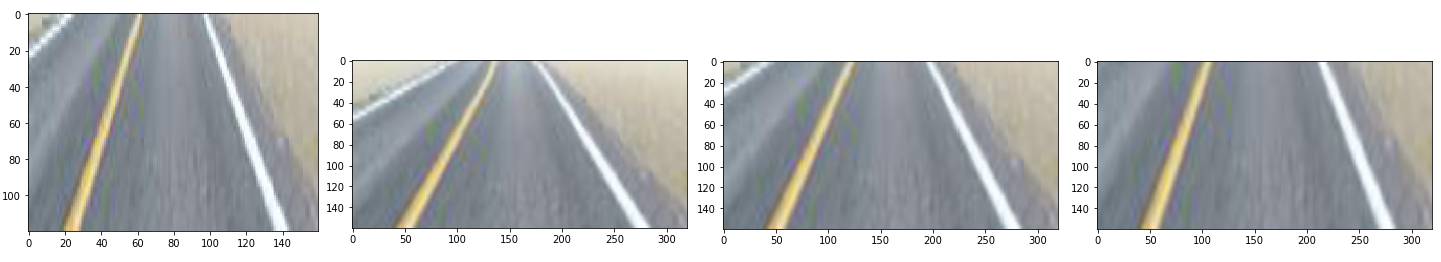
\includegraphics[width=\textwidth]{Figures/nvidia1x1_nvidia2x3_crops.png}
 \caption{Left to right, nvidia1 network crop, nvidia2 network crops at top crop set to 70, 81 and 91 pixels respectively)}
 \label{fig:nvidia1x1_nvidia2x3_crops}
\end{figure}

The network architecture for run 55, aligned with nvidia1 convolutional feature maps, is 24, 32, 64, 64 and 64 feature maps in the convolutional layers (conv2d\_ 1 through conv2d\_ 5):

\begin{verbatim}
_________________________________________________________________
Layer (type)                 Output Shape              Param #   
=================================================================
img_in (InputLayer)          [(None, 66, 200, 3)]      0         
_________________________________________________________________
lambda (Lambda)              (None, 66, 200, 3)        0         
_________________________________________________________________
conv2d_1 (Conv2D)            (None, 31, 98, 24)        1824      
_________________________________________________________________
dropout (Dropout)            (None, 31, 98, 24)        0         
_________________________________________________________________
conv2d_2 (Conv2D)            (None, 14, 47, 32)        19232     
_________________________________________________________________
dropout_1 (Dropout)          (None, 14, 47, 32)        0         
_________________________________________________________________
conv2d_3 (Conv2D)            (None, 5, 22, 64)         51264     
_________________________________________________________________
dropout_2 (Dropout)          (None, 5, 22, 64)         0         
_________________________________________________________________
conv2d_4 (Conv2D)            (None, 3, 20, 64)         36928     
_________________________________________________________________
dropout_3 (Dropout)          (None, 3, 20, 64)         0         
_________________________________________________________________
conv2d_5 (Conv2D)            (None, 1, 18, 64)         36928     
_________________________________________________________________
dropout_4 (Dropout)          (None, 1, 18, 64)         0         
_________________________________________________________________
flattened (Flatten)          (None, 1152)              0         
_________________________________________________________________
dense (Dense)                (None, 100)               115300    
_________________________________________________________________
dense_1 (Dense)              (None, 50)                5050      
_________________________________________________________________
steering_throttle (Dense)    (None, 2)                 102       
=================================================================
Total params: 266,628
Trainable params: 266,628
Non-trainable params: 0
_________________________________________________________________
[(None, 66, 200, 3)]
(None, 66, 200, 3)
(None, 31, 98, 24)
(None, 31, 98, 24)
(None, 14, 47, 32)
(None, 14, 47, 32)
(None, 5, 22, 64)
(None, 5, 22, 64)
(None, 3, 20, 64)
(None, 3, 20, 64)
(None, 1, 18, 64)
(None, 1, 18, 64)
(None, 1152)
(None, 100)
(None, 50)
(None, 2)    
\end{verbatim}

%%%%%%%%%%%%%%%%%%%%%%%%%%%%%%%%%%%%%%%%%%%%%%%%%%%%%%%%%%%%%%%%%%%%%%%%%%%%%
% RUN 56
%%%%%%%%%%%%%%%%%%%%%%%%%%%%%%%%%%%%%%%%%%%%%%%%%%%%%%%%%%%%%%%%%%%%%%%%%%%%%
\subsection{Run 56 - 20201207170938\_ nvidia2.h5}
\label{app_res:56}
\begin{verbatim}
Commit: 8f163e9
Model: nvidia2
Outputs: 2
Dataset: genTrack
Command: Assumed to be the same as previous, which can be backtracked to run 50:
Command: python train.py
--model=nvidia2
--outdir=../trained_models
--epochs=5
--inputs=../dataset/unity/genTrack/*.jpg
--aug=True
--preproc=True

Environment: simbox
Comment: Changed top crop for nvidia2

$ git diff 28ea337..8f163e9 conf.py
diff --git a/src/conf.py b/src/conf.py
index 0ccb633..0b97b8e 100644
--- a/src/conf.py
+++ b/src/conf.py
@@ -42,10 +42,10 @@ NVIDIA1 = 'nvidia1' # a.k.a. TawnNet
 nvidia1_img_dims = [160,120,3,160,120,60,-25]
 # NVIDIA2
 NVIDIA2 = 'nvidia2' # a.k.a. NaokiNet
-nvidia2_img_dims = [320,160,3,200,66,70,-35]
+nvidia2_img_dims = [320,160,3,200,66,81,-35]
 # NVIDIA_BASELINE
 NVIDIA_BASELINE = 'nvidia_baseline' # a.k.a. NaokiNet
-nvidia_baseline_img_dims = [320,160,3,200,66,70,-35]
+nvidia_baseline_img_dims = [320,160,3,200,66,91,-35]

\end{verbatim}

Another crash (\url{https://youtu.be/I3gkoO1yWkk}), changed top crop to 81 in conf.py.

%%%%%%%%%%%%%%%%%%%%%%%%%%%%%%%%%%%%%%%%%%%%%%%%%%%%%%%%%%%%%%%%%%%%%%%%%%%%%
% RUN 57
%%%%%%%%%%%%%%%%%%%%%%%%%%%%%%%%%%%%%%%%%%%%%%%%%%%%%%%%%%%%%%%%%%%%%%%%%%%%%
\subsection{Run 57 - 20201207175205\_ nvidia2.h5}
\label{app_res:57}
\begin{verbatim}
Commit: 485d845
Model: nvidia2
Outputs: 2
Dataset: genTrack
Command:
python train.py
--model=nvidia2
--outdir=../trained_models
--epochs=5
--inputs=../dataset/unity/genTrack/*.jpg
--aug=True
--preproc=True

Environment: simbox
Comment: Same as run 56, done as sanity check. Might have messed up the 
predict_client.py parameters in 56. This model almost goes off the track on the first
corner but actually gets around the track and works with a 81 top crop.

python predict_client.py 
--model=../trained_models/nvidia2/20201207175205_nvidia2.h5 
--modelname=nvidia2 --record=True --modelname=nvidia2
\end{verbatim}

This actually managed to get around the track (\url{https://youtu.be/Vqd2W39CwdA}.
Investigating the logs for the run 57 model:
\begin{verbatim}
/trained_models/nvidia2(master)$ ls -l *20201207175205*
-rw-rw-r-- 1 simbox simbox   41146 Dec  7 17:53 20201207175205_nvidia2_accuracy.png
-rw-rw-r-- 1 simbox simbox 3278432 Dec  7 17:53 20201207175205_nvidia2.h5
-rw-rw-r-- 1 simbox simbox     258 Dec  7 17:53 20201207175205_nvidia2.history
-rw-rw-r-- 1 simbox simbox     195 Dec  7 17:53 20201207175205_nvidia2.log

$ cat 20201207175205_nvidia2.log
Model name: ../trained_models/nvidia2/20201207175205_nvidia2.h5
Total training time: 0:01:41
Training loss: 0.028
Validation loss: 0.014
Training accuracy: 0.716
Validation accuracy: 0.768
\end{verbatim}
And the equivalent for run 56:
\begin{verbatim}
/trained_models/nvidia2(master)$ ls -l *20201207170938*
-rw-rw-r-- 1 simbox simbox   42312 Dec  7 17:11 20201207170938_nvidia2_accuracy.png
-rw-rw-r-- 1 simbox simbox 3278432 Dec  7 17:11 20201207170938_nvidia2.h5
-rw-rw-r-- 1 simbox simbox     258 Dec  7 17:11 20201207170938_nvidia2.history
-rw-rw-r-- 1 simbox simbox     195 Dec  7 17:11 20201207170938_nvidia2.log

/trained_models/nvidia2(master)$ cat 20201207170938_nvidia2.log
Model name: ../trained_models/nvidia2/20201207170938_nvidia2.h5
Total training time: 0:01:40
Training loss: 0.031
Validation loss: 0.016
Training accuracy: 0.689
Validation accuracy: 0.772
\end{verbatim}
Looking at the training history for run 56 (Figure \ref{fig:20201207175205_nvidia2_accuracy}) and run 57 (Figure \ref{fig:20201207170938_nvidia2_accuracy}):

\begin{figure}[ht]
 \centering 
 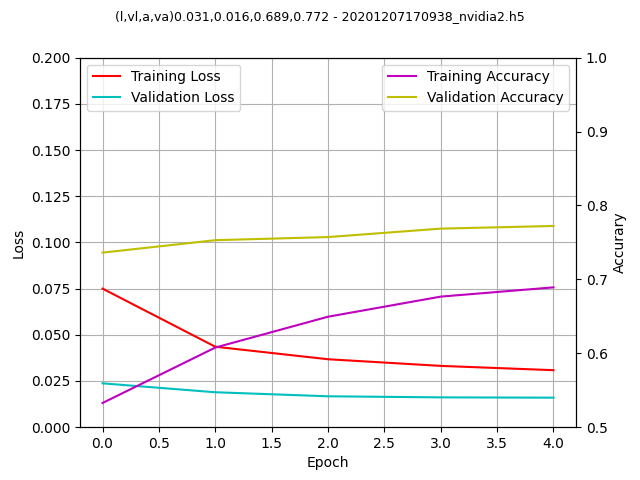
\includegraphics[width=\textwidth]{Figures/20201207170938_nvidia2_accuracy.png}
 \caption{nvidia2 20201207170938\_ nvidia2.h5 (Run 56) model training accuracy for 5 epochs. Refer to \ref{fig:20201207175205_nvidia2_accuracy} for explanation of plot title}
 \label{fig:20201207170938_nvidia2_accuracy} 
\end{figure}

\begin{figure}[ht]
 \centering 
 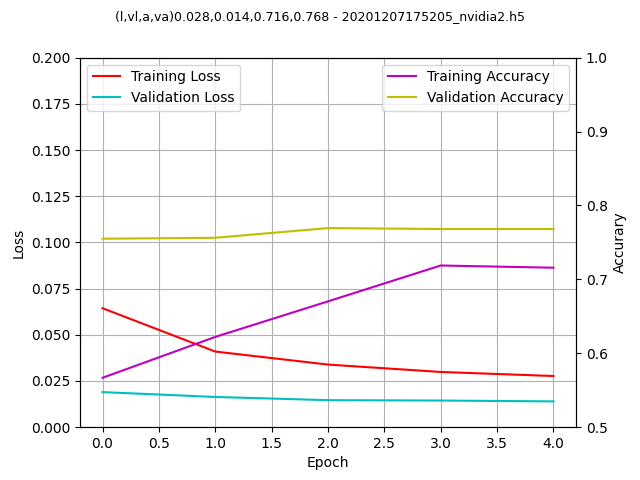
\includegraphics[width=\textwidth]{Figures/20201207175205_nvidia2_accuracy.png}
 \caption{nvidia2 20201207175205\_ nvidia2.h5 (Run 57) model training accuracy for 5 epochs showing in the title the training loss (l), validation loss (vl), training accuracy (a) and validation accuracy (va) recorded for the last (5th - zero indexed) epoch (0.028, 0.014, 0.716 and 0.768, respectively.}
 \label{fig:20201207175205_nvidia2_accuracy} 
\end{figure}

As a final sanity check, a rerun of the inference time drive is done for both models (Run 56 and Run 57, generating the video only from tcpflow data:
\begin{verbatim}
# Run 56
# record tcpflow log
$ sudo tcpflow -i lo -c port 9091 >
../trained_models/nvidia2/tcpflow/20201207170938_Rerun_56_nvidia2.log
# predict
$ python predict_client.py 
--model=../trained_models/nvidia2/20201207170938_nvidia2.h5 --modelname=nvidia2
# make video - had to copy augmentation.py and conf.py to utils (at commit c4158dd), where MakeVideo.py now
# lives
$ python MakeVideo.py 
--filename=../../trained_models/nvidia2/tcpflow/20201207170938_Rerun_56_nvidia2.log
--model="20201207170938_nvidia2.h5"
\end{verbatim}
This produced video \url{https://youtu.be/XGA2oL8QVms} which matches run 56.  
  
Now the same for run 57:
\begin{verbatim}
# Run 57
# record tcpflow log
$ sudo tcpflow -i lo -c port 9091 >
../trained_models/nvidia2/tcpflow/20201207175205_Rerun_57_nvidia2.log
# predict
$ python predict_client.py 
--model=../trained_models/nvidia2/20201207175205_nvidia2.h5 --modelname=nvidia2
# make video - had to copy augmentation.py and conf.py to utils, where MakeVideo.py now
# lives
$ python MakeVideo.py 
--filename=../../trained_models/nvidia2/tcpflow/20201207175205_Rerun_57_nvidia2.log
--model="20201207170938_nvidia2.h5"
\end{verbatim}
This produced video \url{https://youtu.be/cUDiz7v_o3Y} which matches run 57. The result is
mystifying, as it succeeds and precedes a succession of failed nvidia2 architecture runs until the (in hindsight) best "wet" performing model produced in Run 62 \ref{app_res:62} ). One possibility is that the
last 10-unit hidden layer had been commented in for run 57, then commented out, with no commit to show the change. The 10-unit hidden layer made "a", perhaps "the" difference in run 62 \ref{app_res:62}.
% TODO Add to results, after a succession of experiments changing top crop values,
% dropout layers, dropout values and normalizing schemes, a best nvidia2 model
% was produced
%%%%%%%%%%%%%%%%%%%%%%%%%%%%%%%%%%%%%%%%%%%%%%%%%%%%%%%%%%%%%%%%%%%%%%%%%%%%%
% RUN 58
%%%%%%%%%%%%%%%%%%%%%%%%%%%%%%%%%%%%%%%%%%%%%%%%%%%%%%%%%%%%%%%%%%%%%%%%%%%%%
\subsection{Run 58 - 20201207184329\_ nvidia2.h5}
\label{app_res:58}
\begin{verbatim}
Commit: 196f820
Model: nvidia2
Outputs: 2
Dataset: genTrack
Command:
python train.py 
--model=nvidia2
--outdir=../trained_models
--epochs=5
--inputs=../dataset/unity/genTrack/*.jpg
--aug=True
--preproc=True
Environment: simbox
Comment: top crop set to 77. 
Model drove off the road.

Inference time prediction:

$ python predict_client.py ../trained_models/nvidia2/20201207184329_nvidia2.h5
--modelname=nvidia2 --record=True --modelname=nvidia2
\end{verbatim}

Top crop set to 77, drove off the road (\url{https://youtu.be/jHWX7bi5Okw}).

%%%%%%%%%%%%%%%%%%%%%%%%%%%%%%%%%%%%%%%%%%%%%%%%%%%%%%%%%%%%%%%%%%%%%%%%%%%%%
% RUN 59
%%%%%%%%%%%%%%%%%%%%%%%%%%%%%%%%%%%%%%%%%%%%%%%%%%%%%%%%%%%%%%%%%%%%%%%%%%%%%
\subsection{Run 58 - 20201207185525\_ nvidia2.h5}
\label{app_res:58}
\begin{verbatim}
Commit: 0cc41e7
Model: nvidia2
Outputs: 2
Dataset: genTrack   
Command:
python train.py 
--model=nvidia2
--outdir=../trained_models
--epochs=5
--inputs=../dataset/unity/genTrack/*.jpg
--aug=True
--preproc=True
Environment: simbox

Comment: top crop set to 83. Drove off the road

$ python predict_client.py 
--model=../trained_models/nvidia2/20201207185525_nvidia2.h5 --modelname=nvidia2 
--record=True --modelname=nvidia2

\end{verbatim}
Video: \url{https://youtu.be/dkV0Tbfwr9Q}

%%%%%%%%%%%%%%%%%%%%%%%%%%%%%%%%%%%%%%%%%%%%%%%%%%%%%%%%%%%%%%%%%%%%%%%%%%%%%
% RUN 60
%%%%%%%%%%%%%%%%%%%%%%%%%%%%%%%%%%%%%%%%%%%%%%%%%%%%%%%%%%%%%%%%%%%%%%%%%%%%%
\subsection{Run 60 - 20201207190447\_ nvidia2.h5}
\label{app_res:60}
\begin{verbatim}
Commit: f1a5263
Model:  Same as 59
Outputs:  Same as 59
Dataset:  Same as 59
Command: Same as 59

Environment: simbox
Comment: Crash - another simulated car drives off the road.

Prediction:
$ python predict_client.py 
--model=../trained_models/nvidia2/20201207190447_nvidia2.h5 --modelname=nvidia2 
--record=True --modelname=nvidia2
\end{verbatim}

%%%%%%%%%%%%%%%%%%%%%%%%%%%%%%%%%%%%%%%%%%%%%%%%%%%%%%%%%%%%%%%%%%%%%%%%%%%%%
% RUN 61
%%%%%%%%%%%%%%%%%%%%%%%%%%%%%%%%%%%%%%%%%%%%%%%%%%%%%%%%%%%%%%%%%%%%%%%%%%%%%
\subsection{Run 61 - 20201207192309\_ nvidia2.h5 }
\label{app_res:XX}
\begin{verbatim}
Commit: ae4742b
Model:  Same as 59
Outputs:  Same as 59
Dataset:  Same as 59
Command: Same as 59
Comment: Not zero centering pixel values, just normalizing. Crashed.

Investigating the actual changes for the nvidia2 model:

$ git diff --name-only f1a5263..ae4742b
src/conf.py
src/models.py

$ git diff f1a5263..ae4742b conf.py
diff --git a/src/conf.py b/src/conf.py
index e0efddd..d64e228 100644
--- a/src/conf.py
+++ b/src/conf.py
@@ -42,7 +42,7 @@ NVIDIA1 = 'nvidia1' # a.k.a. TawnNet
 nvidia1_img_dims = [160,120,3,160,120,60,-25]
 # NVIDIA2
 NVIDIA2 = 'nvidia2' # a.k.a. NaokiNet
-nvidia2_img_dims = [320,160,3,200,66,83,-35]
+nvidia2_img_dims = [320,160,3,200,66,81,-35]

$ git diff f1a5263..ae4742b models.py
diff --git a/src/models.py b/src/models.py
index adfada8..2539322 100644
--- a/src/models.py
+++ b/src/models.py
@@ -141,21 +141,21 @@ def nvidia_model2(num_outputs):
     row, col, ch = conf.nvidia2_img_dims[conf.IMG_HEIGHT_NET_IDX],
     conf.nvidia2_img_dims[conf.IMG_WIDTH_NET_IDX], \
                    conf.nvidia2_img_dims[conf.IMG_DEPTH_IDX]
 
-    drop = 0.5
+    drop = 0.1
 
     img_in = Input(shape=(row, col, ch), name='img_in')
     x = img_in
     # x = Cropping2D(cropping=((10,0), (0,0)))(x) #trim 10 pixels off top
-    x = Lambda(lambda x: x/127.5 - 1.0)(x) # normalize and re-center
-    # x = Lambda(lambda x: x / 255.0)(x)
+    # x = Lambda(lambda x: x/127.5 - 1.0)(x) # normalize and re-center
+    x = Lambda(lambda x: x / 255.0)(x)
     x = Conv2D(24, (5, 5), strides=(2, 2), activation='elu', name="conv2d_1")(x)
-    # x = Dropout(drop)(x)
-    x = Conv2D(36, (5, 5), strides=(2, 2), activation='elu', name="conv2d_2")(x)
-    # x = Dropout(drop)(x)
+    x = Dropout(drop)(x)
+    x = Conv2D(32, (5, 5), strides=(2, 2), activation='elu', name="conv2d_2")(x)
+    x = Dropout(drop)(x)
     x = Conv2D(48, (5, 5), strides=(2, 2), activation='elu', name="conv2d_3")(x)
-    # x = Dropout(drop)(x)
+    x = Dropout(drop)(x)
     x = Conv2D(64, (3, 3), activation='elu', name="conv2d_4")(x) # default strides=(1,1)
-    # x = Dropout(drop)(x)
+    x = Dropout(drop)(x)
     x = Conv2D(64, (3, 3), activation='elu', name="conv2d_5")(x)
     x = Dropout(drop)(x)

Top crop is set at 81, multiple dropout layers with dropout set at 0.1.
\end{verbatim}
\url{https://youtu.be/5VnNHD0wgFc}


%%%%%%%%%%%%%%%%%%%%%%%%%%%%%%%%%%%%%%%%%%%%%%%%%%%%%%%%%%%%%%%%%%%%%%%%%%%%%
% RUN 62 - One of the best nvidia2 architecture models
%%%%%%%%%%%%%%%%%%%%%%%%%%%%%%%%%%%%%%%%%%%%%%%%%%%%%%%%%%%%%%%%%%%%%%%%%%%%%
\subsection{Run62 - 20201207192948\_ nvidia2.h5}
\label{app_res:62}
\begin{verbatim}
Commit: df953d2
Model:  Same as 59
Outputs:  Same as 59
Dataset:  Same as 59
Command: Same as 59
Environment: same as 59
Comment: Restore last 10 unit fully connected layer. This one drives well around 
Generated Track. This last layer, perhaps together with non-zero centered pixel 
values and multi-dropout layers may have made the difference. Or perhaps just the 
final 10 hidden units? Will probably not have time to test so leaving as 
recommendation for future work i.e. does last ten hidden units before output neurons 
work with zero-centered normalised inputs?

$ python predict_client.pymake up 
--model=../trained_models/nvidia2/20201207192948_nvidia2.h5 --modelname=nvidia2 
--record=True --modelname=nvidia2
\end{verbatim}
\url{https://youtu.be/7-Paz1_PKAo}

%%%%%%%%%%%%%%%%%%%%%%%%%%%%%%%%%%%%%%%%%%%%%%%%%%%%%%%%%%%%%%%%%%%%%%%%%%%%%
% RUN 63
%%%%%%%%%%%%%%%%%%%%%%%%%%%%%%%%%%%%%%%%%%%%%%%%%%%%%%%%%%%%%%%%%%%%%%%%%%%%%
\subsection{Run 63 - 20201207193607\_ nvidia2.h5}
%\label{app_res:63}
\begin{verbatim}
Commit: 3f65201
Model:  Same as 59
Outputs:  Same as 59
Dataset:  Same as 59
Command: Same as 59
Environment: same as 59 
Comment: Only one dropout layer as per original NaokiNet model. Seemed to be
getting around the road ok, until it drove off the road. Otherwise, Very smooth.
Comparable to run 62.

$ python predict_client.py 
--model=../trained_models/nvidia2/20201207193607_nvidia2.h5 --modelname=nvidia2 
--record=True --modelname=nvidia2

\end{verbatim}
Video: \url{https://youtu.be/p2Y6FZX4hNA}

%%%%%%%%%%%%%%%%%%%%%%%%%%%%%%%%%%%%%%%%%%%%%%%%%%%%%%%%%%%%%%%%%%%%%%%%%%%%%
% RUN 64
%%%%%%%%%%%%%%%%%%%%%%%%%%%%%%%%%%%%%%%%%%%%%%%%%%%%%%%%%%%%%%%%%%%%%%%%%%%%%
\subsection{Run 64 - 20201207194331\_ nvidia2.h5}
%\label{app_res:64}
\begin{verbatim}
commit: 3cc0a1bfb8
Model:  Same as 59
Outputs:  Same as 59
Dataset:  Same as 59
Command: Same as 59
Environment: same as 59 
Comment: No Dropout layers. This model although trained on Generated Track data,
drives well on Generated Road circuit.

$ python predict_client.py --model=../trained_models/nvidia2/20201207194331_nvidia2.h5
--modelname=nvidia2 --record=True --modelname=nvidia2

TODO - time allowing, run predictions on Generated Track and compare steering
for networks trained with none, one, and several dropout layers (runs 63, 64
and 49). Or move this paragraph to reflections section.
\end{verbatim}
Video (\url{https://youtu.be/N9xyRizMJvI}) showing the first few hundred frames of model  
nvidia2 20201207194331\_ nvidia2.h5 on the randomly Generated Road circuit.


%%%%%%%%%%%%%%%%%%%%%%%%%%%%%%%%%%%%%%%%%%%%%%%%%%%%%%%%%%%%%%%%%%%%%%%%%%%%%
% RUN 65 - problem here video is the same as Run 66
% although video title (named after file is 20201207193607 nvidia2 h5
% If however we look at video file: 20201207193607_nvidia2.h5'
% it refers to network 20201207193607_nvidia2.h5
%%%%%%%%%%%%%%%%%%%%%%%%%%%%%%%%%%%%%%%%%%%%%%%%%%%%%%%%%%%%%%%%%%%%%%%%%%%%%
\subsection{Run 65 - 20201207194331\_ nvidia2.h5 }
%\label{app_res:65}
\begin{verbatim}
Comment: Duplicate entry, same as 64.
\end{verbatim}
% \url{https://youtu.be/WA2uLtRn3Z0}
% https://youtu.be/WA2uLtRn3Z0 is the same for runs 65 and 66

%%%%%%%%%%%%%%%%%%%%%%%%%%%%%%%%%%%%%%%%%%%%%%%%%%%%%%%%%%%%%%%%%%%%%%%%%%%%%
% RUN 66 - problem here 
%%%%%%%%%%%%%%%%%%%%%%%%%%%%%%%%%%%%%%%%%%%%%%%%%%%%%%%%%%%%%%%%%%%%%%%%%%%%%
\subsection{Run 66 - 20201207193607\_ nvidia2.h5}
\label{app_res:65}
\begin{verbatim}
Comment: Model 63 (only one dropout layer) on Generated Road. Also a bit wobbly but
manages to stay on the road for a while (drop off in the end).
\end{verbatim}
This is a duplicate entry to run 63 - video is \url{https://youtu.be/p2Y6FZX4hNA}
The previously attributed video log \url{https://youtu.be/WA2uLtRn3Z0} refers to an incorrectly labelled upload. 
Another upload was made for run 66 \url{https://youtu.be/v34aJKjeiNs} which is in fact a duplicate to run 63, bar an extra second at the end.


%%%%%%%%%%%%%%%%%%%%%%%%%%%%%%%%%%%%%%%%%%%%%%%%%%%%%%%%%%%%%%%%%%%%%%%%%%%%%
% RUN 67
%%%%%%%%%%%%%%%%%%%%%%%%%%%%%%%%%%%%%%%%%%%%%%%%%%%%%%%%%%%%%%%%%%%%%%%%%%%%%
\subsection{Run 67 - 20201207195804\_ nvidia2.h5}
%\label{app_res:XX}
\begin{verbatim}
Commit: 957d14c
Model:  Same as 59
Outputs:  Same as 59
Dataset:  Same as 59
Command: Same as 59
Environment: same as 59 
Comment: zero centered pixel values, drove off the road. This seems to be
the change that most impacts model performance, followed by image size.

$ git diff 3cc0a1bfb8..957d14c models.py
diff --git a/src/models.py b/src/models.py
index 7d4618e..fc143e2 100644
--- a/src/models.py
+++ b/src/models.py
@@ -146,8 +146,8 @@ def nvidia_model2(num_outputs):
     img_in = Input(shape=(row, col, ch), name='img_in')
     x = img_in
     # x = Cropping2D(cropping=((10,0), (0,0)))(x) #trim 10 pixels off top
-    # x = Lambda(lambda x: x/127.5 - 1.0)(x) # normalize and re-center
-    x = Lambda(lambda x: x / 255.0)(x)
+    x = Lambda(lambda x: x/127.5 - 1.0)(x) # normalize and re-center
+    # x = Lambda(lambda x: x / 255.0)(x)

This nvidia2 model does have the last dense(10) hidden layer:

$ git checkout -b looksee 957d14c
Switched to a new branch 'looksee'
$ cat models.py | grep Dense\(10
(...)
    x = Dense(10, activation='elu')(x) # Added in Naoki's model
(...)

    x = Dense(10, activation='elu')(x) # Added in Naoki's model

Also worth noting, it used elu as activation function for all except output layer.
Prediction:
$ python predict_client.py --model=../trained_models/nvidia2/20201207195804_nvidia2.h5
--modelname=nvidia2 --record=True --modelname=nvidia2

\end{verbatim}
\url{https://youtu.be/ZSgKMGL7azY}

%%%%%%%%%%%%%%%%%%%%%%%%%%%%%%%%%%%%%%%%%%%%%%%%%%%%%%%%%%%%%%%%%%%%%%%%%%%%%
% RUN 68
%%%%%%%%%%%%%%%%%%%%%%%%%%%%%%%%%%%%%%%%%%%%%%%%%%%%%%%%%%%%%%%%%%%%%%%%%%%%%
\subsection{Run 68 - 20201207201157\_ nvidia\_ baseline.h5 }
%\label{app_res:68}
\begin{verbatim}
Commit: b1af57c
Model: nvidia_baseline
Outputs: 2
Dataset: genTrack
Command:
python train.py
--model=nvidia_baseline
--outdir=../trained_models
--epochs=5
--inputs=../dataset/unity/genTrack/*.jpg
--aug=True
--preproc=True
Environment: simbox
Comment: Drove off the road. Looks like geometry of input image must be known.
\end{verbatim}
\url{https://youtu.be/RxcC9tHCVUo}



%%%%%%%%%%%%%%%%%%%%%%%%%%%%%%%%%%%%%%%%%%%%%%%%%%%%%%%%%%%%%%%%%%%%%%%%%%%%%
% RUN 69
%%%%%%%%%%%%%%%%%%%%%%%%%%%%%%%%%%%%%%%%%%%%%%%%%%%%%%%%%%%%%%%%%%%%%%%%%%%%%
\subsection{Run 69 - }
%\label{app_res:69}
\begin{verbatim}
Commit: 4831a1b
Model: nvidia2
Outputs: 2
Dataset: genTrack
Command:
python train.py
--model=nvidia2
--outdir=../trained_models
--epochs=5
--inputs=../dataset/unity/genTrack/*.jpg
--aug=True
--preproc=True
Environment: simbox
Comment: set second convolutional layer to 32 feature maps failed to predict.

    ValueError: Input 0 of layer dense is incompatible with the layer: expected axis -1 of input shape to have value 6656 but received input with shape [None, 1152]

Was still zero centering (sanity checking)

$ python predict_client.py --model=../trained_models/nvidia2/20201102090041_nvidia2.h5  --record=True --modelname=nvidia2


\end{verbatim}

%%%%%%%%%%%%%%%%%%%%%%%%%%%%%%%%%%%%%%%%%%%%%%%%%%%%%%%%%%%%%%%%%%%%%%%%%%%%%
% RUN 70
%%%%%%%%%%%%%%%%%%%%%%%%%%%%%%%%%%%%%%%%%%%%%%%%%%%%%%%%%%%%%%%%%%%%%%%%%%%%%
\subsection{Run 70 - 20201207203451\_ nvidia2.h5 }
%\label{app_res:XX}
\begin{verbatim}
Commit: 5e313d6 
Model: nvidia2
Outputs: 2
Dataset: genTrack   
Command:
python train.py
--model=nvidia2
--outdir=../trained_models
--epochs=5
--inputs=../dataset/unity/genTrack/*.jpg
--aug=True
--preproc=True

Environment: simbox
Comment: Weird how a change in feature map size changes model performance. It is still going ok but not the best.

$ python predict_client.py --model=../trained_models/nvidia2/20201207203451_nvidia2.h5  --record=True --modelname=nvidia2

\end{verbatim}
\url{https://youtu.be/3h_Lp3gtHnw}

%%%%%%%%%%%%%%%%%%%%%%%%%%%%%%%%%%%%%%%%%%%%%%%%%%%%%%%%%%%%%%%%%%%%%%%%%%%%%
% RUN 71 
%%%%%%%%%%%%%%%%%%%%%%%%%%%%%%%%%%%%%%%%%%%%%%%%%%%%%%%%%%%%%%%%%%%%%%%%%%%%%
\subsection{Run 71 - }
%\label{app_res:XX}
\begin{verbatim}
Commit: bc76eb3 
Model: alexnet
Outputs: 2 
Dataset: genTrack
Command:
python train.py
--model=alexnet
--outdir=../trained_models
--epochs=5
--inputs=../dataset/unity/genTrack/*.jpg
--aug=True
--preproc=True

Environment: 
Comment: Error - Input to reshape is a tensor with 495616 values, but the
requested shape requires a multiple of 6336. Need to sort out shapes.
\end{verbatim}

%%%%%%%%%%%%%%%%%%%%%%%%%%%%%%%%%%%%%%%%%%%%%%%%%%%%%%%%%%%%%%%%%%%%%%%%%%%%%
% RUN 72
%%%%%%%%%%%%%%%%%%%%%%%%%%%%%%%%%%%%%%%%%%%%%%%%%%%%%%%%%%%%%%%%%%%%%%%%%%%%%
\subsection{Run 72 - 20201207091932\_ nvidia1.h5 }
%\label{app_res:72}
\begin{verbatim}
Commit: bc76eb3 
Model: nvidia1
Outputs: 2
Dataset: genTrack
Command:
sudo tcpflow -i lo -c port 9091 >
/tmp/20201207091932_nvidia1_light_rain_mult_1_tcpflow.log

$ python predict_client.py
--model=../trained_models/nvidia1/20201207091932_nvidia1.h5 --modelname=nvidia1
--rain='light' --slant=0 --record=True

Environment: simbox
Comment: light rain


\end{verbatim}
\url{https://youtu.be/ulMMgQyMwNI}

%%%%%%%%%%%%%%%%%%%%%%%%%%%%%%%%%%%%%%%%%%%%%%%%%%%%%%%%%%%%%%%%%%%%%%%%%%%%%
% RUN 73
%%%%%%%%%%%%%%%%%%%%%%%%%%%%%%%%%%%%%%%%%%%%%%%%%%%%%%%%%%%%%%%%%%%%%%%%%%%%%
\subsection{Run 73 - 20201207091932\_ nvidia1.h5}
%\label{app_res:73}
\begin{verbatim}
Commit: bc76eb3 
Model: nvidia1
Outputs: 2
Dataset: genTrack
Command:
sudo tcpflow -i lo -c port 9091 >
/tmp/20201207091932_nvidia1_heavy_10_mult_1_tcpflow.log

$ python predict_client.py
--model=../trained_models/nvidia1/20201207091932_nvidia1.h5 --modelname=nvidia1
--rain='heavy' --slant=10 --record=True

Environment: simbox
Comment: heavy rain 10 degree slant
\end{verbatim}
\url{https://youtu.be/Yff1s3RYFSg}

%%%%%%%%%%%%%%%%%%%%%%%%%%%%%%%%%%%%%%%%%%%%%%%%%%%%%%%%%%%%%%%%%%%%%%%%%%%%%
% RUN 74
%%%%%%%%%%%%%%%%%%%%%%%%%%%%%%%%%%%%%%%%%%%%%%%%%%%%%%%%%%%%%%%%%%%%%%%%%%%%%
\subsection{Run 74 - 20201207091932\_ nvidia1.h5}
%\label{app_res:74}
\begin{verbatim}
Commit: 
Model: 
Outputs: 
Dataset: 
Command:
sudo tcpflow -i lo -c port 9091 >
/tmp/20201207091932_nvidia1_torrential_20__mult_1_tcpflow.log

$ python predict_client.py
--model=../trained_models/nvidia1/20201207091932_nvidia1.h5 --modelname=nvidia1
--rain='torrential' --slant=20 --record=True

Environment: simbox
Comment: Torrential rain, 20 degree slant
\end{verbatim}
\url{https://youtu.be/Hn4fXr1a89I}


%%%%%%%%%%%%%%%%%%%%%%%%%%%%%%%%%%%%%%%%%%%%%%%%%%%%%%%%%%%%%%%%%%%%%%%%%%%%%
% RUN 75
%%%%%%%%%%%%%%%%%%%%%%%%%%%%%%%%%%%%%%%%%%%%%%%%%%%%%%%%%%%%%%%%%%%%%%%%%%%%%
\subsection{Run 75 - 20201207091932\_ nvidia1.h5 }
%\label{app_res:75}
\begin{verbatim}
Commit: 4d2c67e
Model: nvidia1
Outputs: 2
Dataset: genTrack
Command:
sudo tcpflow -i lo -c port 9091 > /tmp/20201207091932_nvidia1_light_rain_mult_4_tcpflow.log

$ python predict_client.py --model=../trained_models/nvidia1/20201207091932_nvidia1.h5 --modelname=nvidia1 --rain='light' --slant=0 --record=True

Environment: simbox
Comment: Light rain, intensity multiply 4
\end{verbatim}
\url{https://youtu.be/qdTA5ho5VOE}

%%%%%%%%%%%%%%%%%%%%%%%%%%%%%%%%%%%%%%%%%%%%%%%%%%%%%%%%%%%%%%%%%%%%%%%%%%%%%
% RUN 76
%%%%%%%%%%%%%%%%%%%%%%%%%%%%%%%%%%%%%%%%%%%%%%%%%%%%%%%%%%%%%%%%%%%%%%%%%%%%%
\subsection{Run 76 - 20201207091932\_ nvidia1.h5 }
\label{app_res:76}
\begin{verbatim}
Commit: 4d2c67e
Model: nvidia1
Outputs: 2
Dataset: genTrack
Command:
sudo tcpflow -i lo -c port 9091 > /tmp/20201207091932_nvidia1_heavy_10_mult_4_tcpflow.log

$ python predict_client.py --model=../trained_models/nvidia1/20201207091932_nvidia1.h5 --modelname=nvidia1 --rain='heavy' --slant=10 --record=True

Environment: simbox
Comment: Heavy rain, slant -+10, intensity multiply 4
\end{verbatim}
\url{https://youtu.be/sKyoke3IO84}

%%%%%%%%%%%%%%%%%%%%%%%%%%%%%%%%%%%%%%%%%%%%%%%%%%%%%%%%%%%%%%%%%%%%%%%%%%%%%
% RUN 77
%%%%%%%%%%%%%%%%%%%%%%%%%%%%%%%%%%%%%%%%%%%%%%%%%%%%%%%%%%%%%%%%%%%%%%%%%%%%%
\subsection{Run 77 - 20201207091932\_ nvidia1.h5 }
\label{app_res:77}
\begin{verbatim}
Commit: 4d2c67e
Model: nvidia1
Outputs: 2
Dataset: genTrack
Command:
sudo tcpflow -i lo -c port 9091 > /tmp/20201207091932_nvidia1_torrential_20_mult_4_tcpflow.log

$ python predict_client.py --model=../trained_models/nvidia1/20201207091932_nvidia1.h5 --modelname=nvidia1 --rain='torrential' --slant=20 --record=True

Environment: simbox
Comment: Torrential rain, slant -+20, intensity multiply 4
\end{verbatim}
\url{https://youtu.be/mDjtnnVZdic}

%%%%%%%%%%%%%%%%%%%%%%%%%%%%%%%%%%%%%%%%%%%%%%%%%%%%%%%%%%%%%%%%%%%%%%%%%%%%%
% RUN 78
%%%%%%%%%%%%%%%%%%%%%%%%%%%%%%%%%%%%%%%%%%%%%%%%%%%%%%%%%%%%%%%%%%%%%%%%%%%%%
\subsection{Run 78 - 20201207091932\_ nvidia1.h5 }
\label{app_res:78}
\begin{verbatim}
Commit: 8d3745c 
Outputs: 2
Dataset: genTrack
Command:
sudo tcpflow -i lo -c port 9091 > /tmp/20201207091932_nvidia1_light_rain_mult_8_tcpflow.log

$ python predict_client.py --model=../trained_models/nvidia1/20201207091932_nvidia1.h5 --modelname=nvidia1 --rain='light' --slant=0 --record=True

Environment: simbox
Comment: Light rain, intensity multiply 8
\end{verbatim}
\url{https://youtu.be/31Dt8RafE8o}

%%%%%%%%%%%%%%%%%%%%%%%%%%%%%%%%%%%%%%%%%%%%%%%%%%%%%%%%%%%%%%%%%%%%%%%%%%%%%
% RUN 79
%%%%%%%%%%%%%%%%%%%%%%%%%%%%%%%%%%%%%%%%%%%%%%%%%%%%%%%%%%%%%%%%%%%%%%%%%%%%%
\subsection{Run 79 - 20201207091932\_ nvidia1.h5 }
\label{app_res:79}
\begin{verbatim}
Commit: 8d3745c 
Outputs: 2
Dataset: genTrack
Command:
sudo tcpflow -i lo -c port 9091 > /tmp/20201207091932_nvidia1_heavy_10_mult_8_tcpflow.log

$ python predict_client.py --model=../trained_models/nvidia1/20201207091932_nvidia1.h5 --modelname=nvidia1 --rain='heavy' --slant=20 --record=True

Environment: simbox
Comment: Heavy rain, +-10 degree slant, intensity multiply 8
\end{verbatim}
\url{https://youtu.be/RwWftJeJagY}

%%%%%%%%%%%%%%%%%%%%%%%%%%%%%%%%%%%%%%%%%%%%%%%%%%%%%%%%%%%%%%%%%%%%%%%%%%%%%
% RUN 80
%%%%%%%%%%%%%%%%%%%%%%%%%%%%%%%%%%%%%%%%%%%%%%%%%%%%%%%%%%%%%%%%%%%%%%%%%%%%%
\subsection{Run 80 - 20201207091932\_ nvidia1.h5 }
\label{app_res:80}
\begin{verbatim}
Commit: 8d3745c 
Outputs: 2
Dataset: genTrack
Command:
sudo tcpflow -i lo -c port 9091 > /tmp/20201207091932_nvidia1_torrential_20_mult_8_tcpflow.log

$ python predict_client.py --model=../trained_models/nvidia1/20201207091932_nvidia1.h5 --modelname=nvidia1 --rain='torrential' --slant=20 --record=True

Environment: simbox
Comment: Torrential rain, +-20 degree slant, intensity multiply 8
\end{verbatim}
\url{https://youtu.be/ta40jlqdZ04}

%%%%%%%%%%%%%%%%%%%%%%%%%%%%%%%%%%%%%%%%%%%%%%%%%%%%%%%%%%%%%%%%%%%%%%%%%%%%%
% RUN 81
%%%%%%%%%%%%%%%%%%%%%%%%%%%%%%%%%%%%%%%%%%%%%%%%%%%%%%%%%%%%%%%%%%%%%%%%%%%%%
\subsection{Run 81 - 20201207091932\_ nvidia1.h5}
\label{app_res:81}
\begin{verbatim}
Commit: 356fe8f 
Outputs: 2
Dataset: genTrack
Command:
sudo tcpflow -i lo -c port 9091 > /tmp/20201207091932_nvidia1__no_rain_tcpflow.log

$ python predict_client.py
--model=../trained_models/nvidia1/20201207091932_nvidia1.h5 --modelname=nvidia1 
--record=True
Environment: simbox
Comment: Run to create a tcpflow ground truth file (best steering around lap)
\end{verbatim}

%STOPPED HERE - CONTINUE TOMORROW WITH NVIDIA2, same 9 cases Mult 1,4,8,
%light, heavy, torrential



%%%%%%%%%%%%%%%%%%%%%%%%%%%%%%%%%%%%%%%%%%%%%%%%%%%%%%%%%%%%%%%%%%%%%%%%%%%%%
% RUN 82
%%%%%%%%%%%%%%%%%%%%%%%%%%%%%%%%%%%%%%%%%%%%%%%%%%%%%%%%%%%%%%%%%%%%%%%%%%%%%
\subsection{Run 82 - 20201207192948\_ nvidia2.h5 }
\label{app_res:82}
\begin{verbatim}
Commit: 156e1a3f3bb007cbf7090402a9c276c6a9cc835a
Model: nvidia2 
Outputs: 2
Dataset: genTrack
Command:
python predict_client.py
--model=../trained_models/nvidia2/20201207192948_nvidia2.h5 --modelname=nvidia2 
--record=True
Environment: simbox
Comment: No rain lap for best nvidia2 model
Video: https://youtu.be/iePt2HJPXP0
\end{verbatim}


%%%%%%%%%%%%%%%%%%%%%%%%%%%%%%%%%%%%%%%%%%%%%%%%%%%%%%%%%%%%%%%%%%%%%%%%%%%%%
% RUN 83
%%%%%%%%%%%%%%%%%%%%%%%%%%%%%%%%%%%%%%%%%%%%%%%%%%%%%%%%%%%%%%%%%%%%%%%%%%%%%
\subsection{Run 83 - 20201207192948\_ nvidia2.h5 }
nvidia2 actually managed to get around
\label{app_res:83}
\begin{verbatim}
Commit: 156e1a3f3bb007cbf7090402a9c276c6a9cc835a
Model: nvidia2 
Outputs: 2
Dataset: genTrack
Command:
$ sudo tcpflow -i lo -c port 9091 > 
/tmp/20201207192948_nvidia2_light_rain_mult_1_tcpflow.log

$ python predict_client.py
--model=../trained_models/nvidia2/20201207192948_nvidia2.h5 --modelname=nvidia2 
--record=True --rain='light' slant=0
Environment: simbox
Comment: light rain lap for best nvidia2 model
Video: https://youtu.be/d-yY9M2fO4U
\end{verbatim}

%%%%%%%%%%%%%%%%%%%%%%%%%%%%%%%%%%%%%%%%%%%%%%%%%%%%%%%%%%%%%%%%%%%%%%%%%%%%%
% RUN 84
%%%%%%%%%%%%%%%%%%%%%%%%%%%%%%%%%%%%%%%%%%%%%%%%%%%%%%%%%%%%%%%%%%%%%%%%%%%%%
\subsection{Run 84 - 20201207192948\_ nvidia2.h5 }
nvidia2 actually managed to get around again, practically same path
\label{app_res:84}
\begin{verbatim}
Commit: 156e1a3f3bb007cbf7090402a9c276c6a9cc835a
Model: nvidia2 
Outputs: 2
Dataset: genTrack
Command:
$ sudo tcpflow -i lo -c port 9091 > 
/tmp/20201207192948_nvidia2_heavy_10_mult_1_tcpflow.log

$ python predict_client.py
--model=../trained_models/nvidia2/20201207192948_nvidia2.h5 --modelname=nvidia2 
--record=True --rain='heavy' slant=10
Environment: simbox
Comment: Heavy rain slant 10 lap for best nvidia2 model
Video: https://youtu.be/3AhcVqdV6KM
\end{verbatim}

%%%%%%%%%%%%%%%%%%%%%%%%%%%%%%%%%%%%%%%%%%%%%%%%%%%%%%%%%%%%%%%%%%%%%%%%%%%%%
% RUN 85
%%%%%%%%%%%%%%%%%%%%%%%%%%%%%%%%%%%%%%%%%%%%%%%%%%%%%%%%%%%%%%%%%%%%%%%%%%%%%
\subsection{Run 85 - 20201207192948\_ nvidia2.h5 }

%label{app_res:85}
\begin{verbatim}
Commit: 156e1a3f3bb007cbf7090402a9c276c6a9cc835a
Model: nvidia2 
Outputs: 2
Dataset: genTrack
Command:
$ sudo tcpflow -i lo -c port 9091 > 
/tmp/20201207192948_nvidia2_torrential_20_mult_1_tcpflow.log

$ python predict_client.py
--model=../trained_models/nvidia2/20201207192948_nvidia2.h5 --modelname=nvidia2 
--record=True --rain='torrential' slant=20
Environment: simbox
Comment: Torrential rain slant 20 lap for best nvidia2 model
Video: https://youtu.be/zk6XalCoOrw
\end{verbatim}

%%%%%%%%%%%%%%%%%%%%%%%%%%%%%%%%%%%%%%%%%%%%%%%%%%%%%%%%%%%%%%%%%%%%%%%%%%%%%
% RUN 86
%%%%%%%%%%%%%%%%%%%%%%%%%%%%%%%%%%%%%%%%%%%%%%%%%%%%%%%%%%%%%%%%%%%%%%%%%%%%%
\subsection{Run 86 - 20201207192948\_ nvidia2.h5 }
Same batch of 3 with multiplier set to 4
\label{app_res:86}
\begin{verbatim}
Commit: c501da2
Model: nvidia2 
Outputs: 2
Dataset: genTrack
Command:
$ sudo tcpflow -i lo -c port 9091 > 
/tmp/20201207192948_nvidia2_light_rain_mult_4_tcpflow.log

$ python predict_client.py
--model=../trained_models/nvidia2/20201207192948_nvidia2.h5 --modelname=nvidia2 
--record=True --rain='light' slant=0
Environment: simbox
Comment: light rain lap mult 4 for best nvidia2 model
Video: https://youtu.be/nmD8wnVtdoo
\end{verbatim}

%%%%%%%%%%%%%%%%%%%%%%%%%%%%%%%%%%%%%%%%%%%%%%%%%%%%%%%%%%%%%%%%%%%%%%%%%%%%%
% RUN 87
%%%%%%%%%%%%%%%%%%%%%%%%%%%%%%%%%%%%%%%%%%%%%%%%%%%%%%%%%%%%%%%%%%%%%%%%%%%%%
\subsection{Run 87 - 20201207192948\_ nvidia2.h5 }
Same batch of 3 with multiplier set to 4
\label{app_res:87}
\begin{verbatim}
Commit: c501da2
Model: nvidia2 
Outputs: 2
Dataset: genTrack
Command:
$ sudo tcpflow -i lo -c port 9091 > 
/tmp/20201207192948_nvidia2_heavy_10_mult_4_tcpflow.log

$ python predict_client.py
--model=../trained_models/nvidia2/20201207192948_nvidia2.h5 --modelname=nvidia2 
--record=True --rain='heavy' slant=10
Environment: simbox
Comment: heavy rain slant 10 mult 4
Video: https://youtu.be/LTTNYyDFFDk
\end{verbatim}

%%%%%%%%%%%%%%%%%%%%%%%%%%%%%%%%%%%%%%%%%%%%%%%%%%%%%%%%%%%%%%%%%%%%%%%%%%%%%
% RUN 88
%%%%%%%%%%%%%%%%%%%%%%%%%%%%%%%%%%%%%%%%%%%%%%%%%%%%%%%%%%%%%%%%%%%%%%%%%%%%%
\subsection{Run 88 - 20201207192948\_ nvidia2.h5 }
Same batch of 3 with multiplier set to 4
\label{app_res:88}
\begin{verbatim}
Commit: c501da2
Model: nvidia2 
Outputs: 2
Dataset: genTrack
Command:
$ sudo tcpflow -i lo -c port 9091 > 
/tmp/20201207192948_nvidia2_torrential_20_mult_4_tcpflow.log

$ python predict_client.py
--model=../trained_models/nvidia2/20201207192948_nvidia2.h5 --modelname=nvidia2 
--record=True --rain='torrential' slant=20
Environment: simbox
Comment: torrential rain slant 20 mult 4
Video: https://youtu.be/jBB4q1JK3oA
\end{verbatim}

%%%%%%%%%%%%%%%%%%%%%%%%%%%%%%%%%%%%%%%%%%%%%%%%%%%%%%%%%%%%%%%%%%%%%%%%%%%%%
% RUN 89
%%%%%%%%%%%%%%%%%%%%%%%%%%%%%%%%%%%%%%%%%%%%%%%%%%%%%%%%%%%%%%%%%%%%%%%%%%%%%
\subsection{Run 89 - 20201207192948\_ nvidia2.h5 }
Same batch of 3 with multiplier set to 8
\label{app_res:88}
\begin{verbatim}
Commit: fbd3448
Model: nvidia2 
Outputs: 2
Dataset: genTrack
Command:
$ sudo tcpflow -i lo -c port 9091 > 
/tmp/20201207192948_nvidia2_light_rain_mult_8_tcpflow.log

$ python predict_client.py
--model=../trained_models/nvidia2/20201207192948_nvidia2.h5 --modelname=nvidia2 
--record=True --rain='light' slant=0
Environment: simbox
Comment: light rain slant 0 mult 8
Video: https://youtu.be/qY8eL-9V-hM
\end{verbatim}

%%%%%%%%%%%%%%%%%%%%%%%%%%%%%%%%%%%%%%%%%%%%%%%%%%%%%%%%%%%%%%%%%%%%%%%%%%%%%
% RUN 90
%%%%%%%%%%%%%%%%%%%%%%%%%%%%%%%%%%%%%%%%%%%%%%%%%%%%%%%%%%%%%%%%%%%%%%%%%%%%%
\subsection{Run 90 - 20201207192948\_ nvidia2.h5 }
Same batch of 3 with multiplier set to 8
\label{app_res:90}
\begin{verbatim}
Commit: fbd3448
Model: nvidia2 
Outputs: 2
Dataset: genTrack
Command:
$ sudo tcpflow -i lo -c port 9091 > 
/tmp/20201207192948_nvidia2_heavy_10_mult_8_tcpflow.log

$ python predict_client.py
--model=../trained_models/nvidia2/20201207192948_nvidia2.h5 --modelname=nvidia2 
--record=True --rain='heavy' slant=10
Environment: simbox
Comment: heavy rain slant 10 mult 8
Video: https://youtu.be/1PpfHLwOx9M
\end{verbatim}

%%%%%%%%%%%%%%%%%%%%%%%%%%%%%%%%%%%%%%%%%%%%%%%%%%%%%%%%%%%%%%%%%%%%%%%%%%%%%
% RUN 91
%%%%%%%%%%%%%%%%%%%%%%%%%%%%%%%%%%%%%%%%%%%%%%%%%%%%%%%%%%%%%%%%%%%%%%%%%%%%%
\subsection{Run 91 - 20201207192948\_ nvidia2.h5 }
Same batch of 3 with multiplier set to 8
\label{app_res:91}
\begin{verbatim}
Commit: fbd3448
Model: nvidia2 
Outputs: 2
Dataset: genTrack
Command:
$ sudo tcpflow -i lo -c port 9091 > 
/tmp/20201207192948_nvidia2_torrential_20_mult_8_tcpflow.log

$ python predict_client.py
--model=../trained_models/nvidia2/20201207192948_nvidia2.h5 --modelname=nvidia2 
--record=True --rain='torrential' slant=20
Environment: simbox
Comment: Torrential rain slant 20 mult 8
Video: https://youtu.be/W1eRN5DWPXw
\end{verbatim}

%%%%%%%%%%%%%%%%%%%%%%%%%%%%%%%%%%%%%%%%%%%%%%%%%%%%%%%%%%%%%%%%%%%%%%%%%%%%%
% RUN 92
%%%%%%%%%%%%%%%%%%%%%%%%%%%%%%%%%%%%%%%%%%%%%%%%%%%%%%%%%%%%%%%%%%%%%%%%%%%%%
\subsection{Run 92 - 20201209001926\_ nvidia1.h5 }
%\label{app_res:92}
\begin{verbatim}
Commit: 20201209001926_nvidia1.h5

Model: nvidia1 
Outputs: 2
Dataset: genRoad
Command:
python train.py
--model=nvidia1
--outdir=../trained_models
--epochs=100
--inputs=../dataset/unity/genRoad/*.jpg
--aug=True
--preproc=True

Epoch 42/100
3229/3229 [==== (...)

Total training time: 6:35:44
Training loss: nan
Validation loss: nan
Training accuracy: 0.206
Validation accuracy: 0.204

Environment: simbox
Comment: Very wobbly on the road

python predict_client.py --model=../trained_models/nvidia1/20201209001926_nvidia1.h5 --modelname=nvidia1
\end{verbatim}

Starts well then wobbles and goes off road (\url{https://youtu.be/K5FmPq0_OdE})
\begin{figure}[ht]
 \centering 
 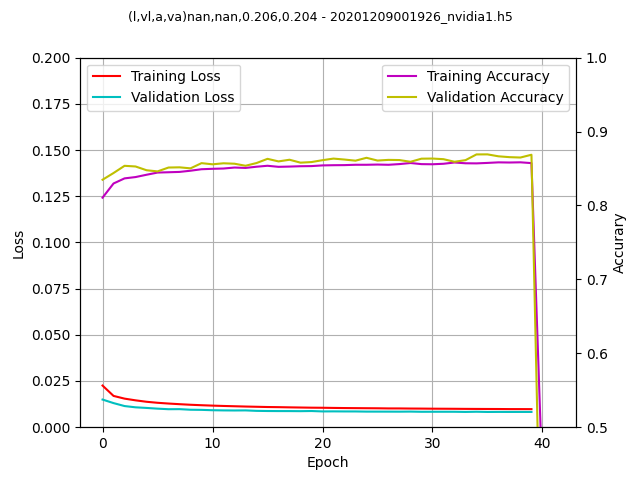
\includegraphics[width=\textwidth]{Figures/20201209001926_nvidia1_accuracy.png}
 \caption{nvidia1 trained on genRoad data for 100 epochs - stopped at 42 (best model saved)}
 \label{fig:20201209001926_nvidia1_accuracy} 
\end{figure}


%%% RUN 93 NVIDIA1 GEN ROAD 5 EPOCHS - STOPPED HERE - DOCUMENT
\begin{verbatim}
Epoch 4/5
3232/3232 [==============================] - 560s 173ms/step - loss: 0.0142 - 
acc: 0.8396 - val_loss: 0.0106 - val_acc: 0.8559
Epoch 5/5
3232/3232 [==============================] - 560s 173ms/step - loss: 0.0136 - 
acc: 0.8422 - val_loss: 0.0101 - val_acc: 0.8494
    
\end{verbatim}

%%%%%%%%%%%%%%%%%%%%%%%%%%%%%%%%%%%%%%%%%%%%%%%%%%%%%%%%%%%%%%%%%%%%%%%%%%%%%
% RUN 93
%%%%%%%%%%%%%%%%%%%%%%%%%%%%%%%%%%%%%%%%%%%%%%%%%%%%%%%%%%%%%%%%%%%%%%%%%%%%%
\subsection{Run 93 - 20201209221402\_ nvidia1.h5 }
%\label{app_res:93}
\begin{verbatim}
Commit: 173d74b
Model: nvidia1
Outputs: 2
Dataset: genRoad
Command:
python train.py
--model=nvidia1
--outdir=../trained_models
--epochs=5
--inputs=../dataset/unity/genRoad/*.jpg
--aug=True
--preproc=True
Environment: simbox
Comment: Same results training for 5 epochs (run 93) and 100 epochs (run 92).

sudo tcpflow -i lo -c port 9091 >
../trained_models/nvidia1/tcpflow/20201209221402_nvidia1_genRoad_dry.log

python3 predict_client.py 
--model=../trained_models/nvidia1/20201209221402_nvidia1.h5 --record=True
\end{verbatim}

Video: \url{https://youtu.be/L6I84lpoAyI}. Starts straight, then wobbles. 
Figure \ref{fig:20201209221402_nvidia1_genRoad_dry} shows the erratic steering starting after frame 100.
\begin{figure}[ht]
 \centering 
 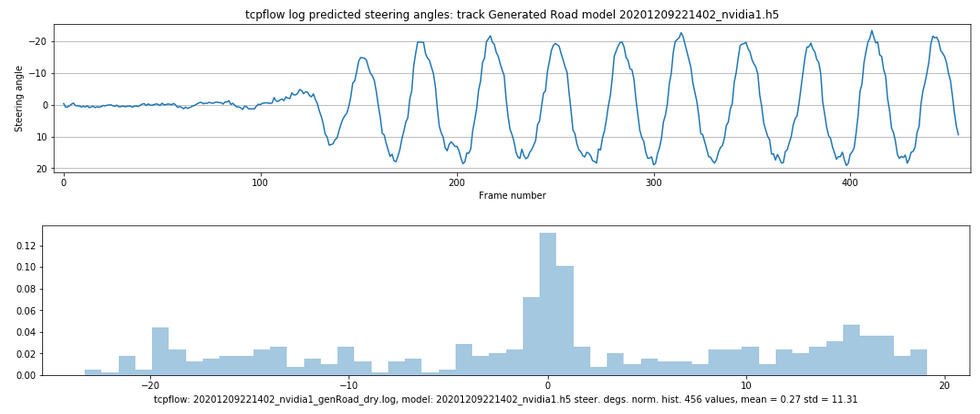
\includegraphics[width=\textwidth]{Figures/20201209221402_nvidia1_genRoad_dry.png}
 \caption{nvidia1 trained on genRoad data for 5 epochs - same results as trained with 100 epochs}
 \label{fig:20201209221402_nvidia1_genRoad_dry} 
\end{figure}

%%%%%%%%%%%%%%%%%%%%%%%%%%%%%%%%%%%%%%%%%%%%%%%%%%%%%%%%%%%%%%%%%%%%%%%%%%%%%
% RUN 94 - 20201207192948_nvidia2.h5
%%%%%%%%%%%%%%%%%%%%%%%%%%%%%%%%%%%%%%%%%%%%%%%%%%%%%%%%%%%%%%%%%%%%%%%%%%%%%
\subsection{Run 94 - 20201207192948\_ nvidia2.h5 }
\label{app_res:94}
\begin{verbatim}
Commit: b0b10e3
Model: nvidia2
Outputs: 2 
Dataset: genTrack
Command: Same as 59
Environment: simbox
Comment: Running a prediction on genRoad data with model trained on genTrack data. Drives quite smoothly. Recommendation for future work: investigate why this is the case, model trained on genTrack drives well on genRoad.

sudo tcpflow -i lo -c port 9091 > ../trained_models/nvidia2/tcpflow/20201207192948_nvidia2_dry_genRoad.log

python3 predict_client.py --model=../trained_models/nvidia2/20201207192948_nvidia2.h5 --record=True --modelname=nvidia2

\end{verbatim}
Video: \url{https://youtu.be/EhTCJ_e-RpM}. 

Figure \ref{fig:20201207192948_nvidia2_dry_genRoad} shows the smoother steering starting centered around 0 degrees, as well as as more even spread in the histogram.
\begin{figure}[ht]
 \centering 
 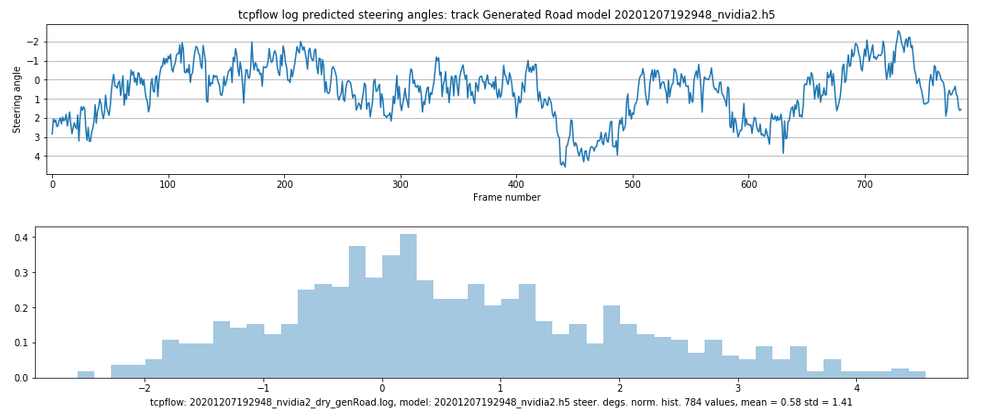
\includegraphics[width=\textwidth]{Figures/20201207192948_nvidia2_dry_genRoad.png}
 \caption{nvidia2 trained on genTrack dataset (from the Generated Track circuit) driving well on the randomly generated Generated Road circuit shown in figure \ref{fig:run-93-94-generated-road}}
 \label{fig:20201207192948_nvidia2_dry_genRoad} 
\end{figure}

Figure \ref{fig:run-93-94-generated-road} shows a randomly Generated Road used for runs 93 and 94, where the first few hundred frames go to near the top left of the circuit (long right 180 degree turn) shown in detail on right. The predicted steering angles shown in Figure  \ref{fig:20201207192948_nvidia2_dry_genRoad} for the well performing nvidia2 20201207192948\_ nvidia2.h5 model, show the majority of values in the positive range, as the simulated vehicle follows the road and takes a right turn to do so.

\begin{figure}[ht]
 \centering 
 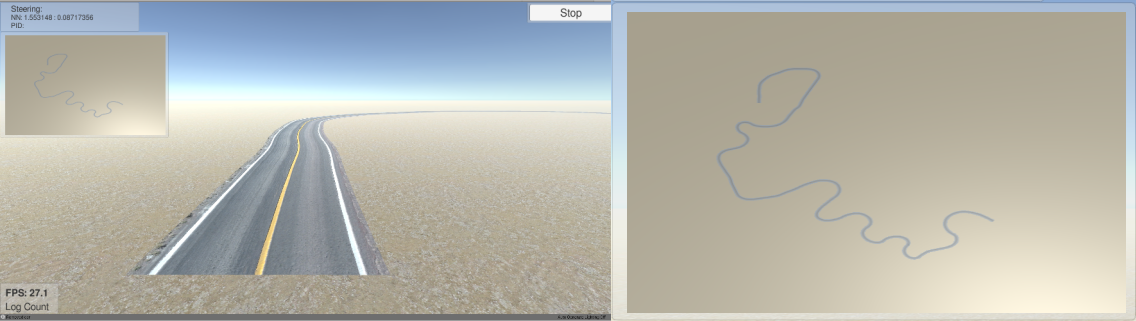
\includegraphics[width=\textwidth]{Figures/run-93-94-generated-road.png}
 \caption{The randomly generated Generated Road circuit used in runs 93 and 94.}
 \label{fig:run-93-94-generated-road} 
\end{figure}


%%%%%%%%%%%%%%%%%%%%%%%%%%%%%%%%%%%%%%%%%%%%%%%%%%%%%%%%%%%%%%%%%%%%%%%%%%%%%
% RUN 95 - 20201207192948_nvidia2.h5
%%%%%%%%%%%%%%%%%%%%%%%%%%%%%%%%%%%%%%%%%%%%%%%%%%%%%%%%%%%%%%%%%%%%%%%%%%%%%
\subsection{Run 95 - 20201207192948\_ nvidia2.h5 }
%\label{app_res:95}
\begin{verbatim}
Commit: c4158dd
Model: nvidia2
Outputs: 2
Dataset: genTrack   
Command: same as 59
Environment: simbox
Comment: One of the best nvidia2 models self-driving the entirety of a randomly
generated road.

\end{verbatim}
Video: \url{https://youtu.be/z9nILq9dQfI}.

Figure \ref{fig:20201207192948_nvidia2_dry_genRoad_full} showing steering angles and normalized histogram plots. This run (95) is much smoother than run 93 (\ref{app_res:93}) which seems also to be suggested in the distributions shown in the related histograms, although run 93 represents a much shorter section.
\begin{figure}[ht]
 \centering 
 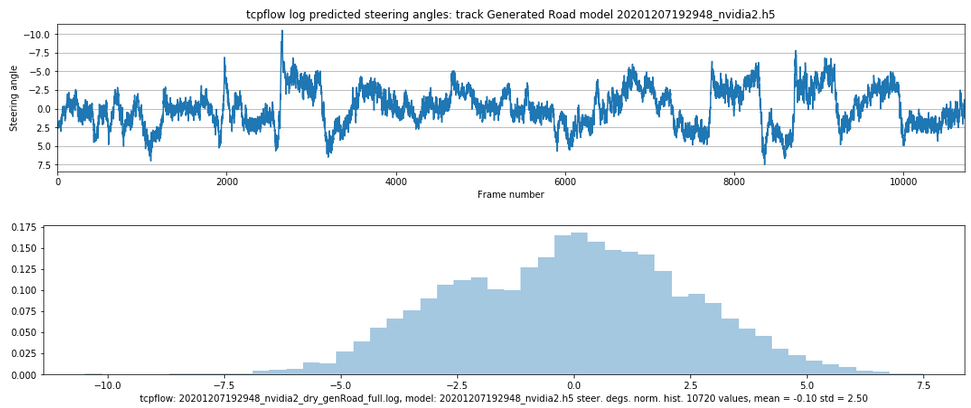
\includegraphics[width=\textwidth]{Figures/20201207192948_nvidia2_dry_genRoad_full.png}
 \caption{Steering angle and normalized histogram plots of the 20201207192948\_ nvidia2.h5 model driving the full length of Generated Track presented in figure \ref{fig:run-93-94-generated-road} }
 \label{fig:20201207192948_nvidia2_dry_genRoad_full} 
\end{figure}


%%%%%%%%%%%%%%%%%%%%%%%%%%%%%%%%%%%%%%%%%%%%%%%%%%%%%%%%%%%%%%%%%%%%%%%%%%%%%
% RUN XX - TEMPLATE
%%%%%%%%%%%%%%%%%%%%%%%%%%%%%%%%%%%%%%%%%%%%%%%%%%%%%%%%%%%%%%%%%%%%%%%%%%%%%
\subsection{Run XX -  }
%\label{app_res:XX}
\begin{verbatim}
Commit:
Model: 
Outputs: 
Dataset: 
Command:
Environment: 
Comment: 
\end{verbatim}





